\chapter{A new approach to STM analysis}
Conventional methods in analyzing grid maps from STM measurements face multiple fundamental  challenges. Recently, thanks to the maturation of optimization algorithms, a convolution data model for STM datasets was proposed by Cheung et al.\cite{cheungDictionaryLearningFouriertransform2020} and shows great potential. However,  despite its success in addressing some of the challenges, key shortcomings exist that prevent it being useful in most of the specimens studied by STM. Here, we introduce a more general model that extends the convolution framework, we then showcase its performance with various benchmark tests, and apply it to real STM data as an illustration.  

\section{Challenges of the conventional analysis methods}
In this section, I will briefly introduce the conventional analysis methods used in the field, 2 fundamental challenges faced with the current method, and discuss the existing approaches to address these challenges and their limitations. 

Fundamentally, experimental results capture the interaction between the probe and the target; To distill the scientific essence presented in the results, complex analysis are usually required. In the case of microscopy measurements like STM, conventional methods like \ac{FT} are commonly used. %todo: add citations on examples of FT microscopy.
The \ac{FT} reveals characteristic wavelengths and provides insights to the underlying scientific theories of the specimen studied; This is particularly true in cases where the microscopy results contain near perfect periodic features, but when aperiodic signals are presented, the \ac{FT} is less ideal and suffers from loss of information. 

There are 2 specific challenges in QPI analysis with conventional \ac{FT} method we would like to focus on, the speckle problem, and the demixing problem. We will also establish their mathematical formulations, which will lead to the convolutional data model we present later. 

\subsection{The Speckle problem}
As introduced in the end of Ch5 and theorized explicitly in Equation \ref{eq.539}, when we take \ac{FT} of the grid map on multiple occurrence of defects, we get speckles on the \ac{FT-STS}; The problem is that the spatial distribution information of the defect location manifest as undesirable patterns in the \ac{FT} space, and makes the QPI pattern hard to interpret.

Therefore, to address the challenge of speckles is to disentangle the spatial information from the \ac{QPI} pattern, and this can be formulated mathematically as a deconvolution problem. 

\par \noindent Recall that we can write the modulation of \ac{LDOS} $\delta \rho$ from multiple defects as:
\begin{equation}
	\delta \rho(\mathbf{x}, \omega) = \sum_{j=1}^{N}c_j \cdot \delta \rho_0(\mathbf{x}-\mathbf{x_j},\omega),
\end{equation}
\noindent where $\delta \rho_0$ is the \ac{LDOS} modulation from individual defect located at at $\mathbf{x_j}$. We can further separate the spatial information by utilizing a Kronecker delta $\Delta(\mathbf{u})$, so that $\Delta(\mathbf{u})=1$ if $\mathbf{u} = 0$, and $\Delta(\mathbf{u})=0$ elsewhere: 
\begin{equation}
	\sum_{j=1}^{N}c_j \cdot \delta \rho_0(\mathbf{x}-\mathbf{x_j},\omega) = \sum_{\mathbf{u}} \delta \rho_0(\mathbf{x}-\mathbf{u},\omega)\cdot(\sum_{j=1}^{N} c_j \cdot \Delta(\mathbf{u-x_j})).
\end{equation}
\noindent We can then construct a convolution sum between the individual \ac{QPI} pattern and the spatial information by defining a defect location function $D(\mathbf{x}) \equiv \sum_{j=1}^{N} c_j \cdot \Delta(\mathbf{u-x_j})$, we have: 
\begin{equation}
	\delta \rho(\mathbf{x}, \omega) =  \sum_{\mathbf{u}} \delta \rho_0(\mathbf{x}-\mathbf{u},\omega)\cdot D(\mathbf{u}) = (\delta \rho_0 *D)(\mathbf{x}, \omega).
\end{equation}

We illustrate this convolution in Fig. \ref{fig:ch6_decon}; First, we use $\delta \rho_0$ simulated in Ch.5.2 as the \ac{QPI} pattern from an single defect, we then randomly generate a binary defect location map given a defect density, and use the convolution sum to construct an observation Y. To unify the language, we will refer the single defect \ac{QPI} pattern as a kernel, denoted as A; and the defect location map as an activation map, denoted as X. Therefore, our goal is that given $Y = A * X$, we want to reconstruct A and X. 

\begin{figure}
	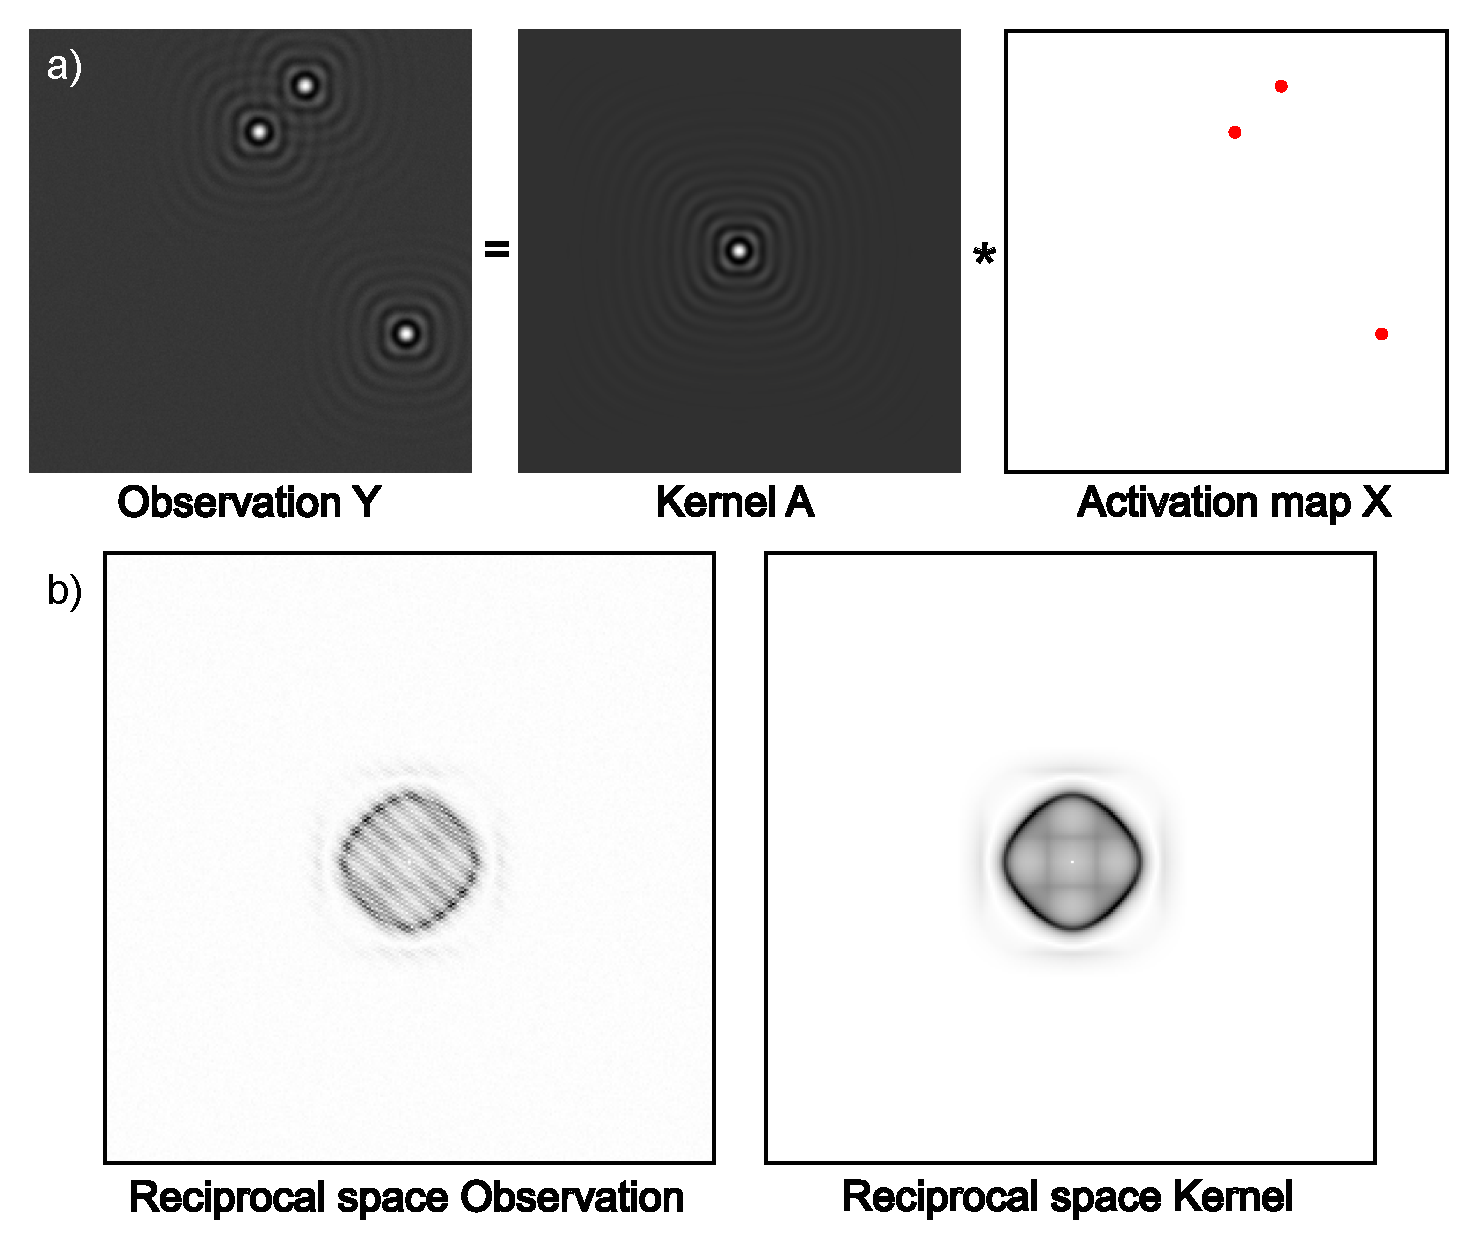
\includegraphics[width= \textwidth]{Ch6_deconvolution.pdf} 
	\centering
	\caption{}
	\label{fig:ch6_decon}
\end{figure}

\subsection{The Demixing problem}
%todo: how should I include the general motivation of demxing? or is it enough here? 
Materials normally exhibit multiple types of defects, and these defects can present different scattering features; Many QPI measurements have exploited the mechanisms of selectivity scattering channels across a wide variety of materials, such as the sign variation of the superconducting order parameter, the spin and orbital texture of topological bands, etc. However, there are only limited approaches to analyze and disentangle defect dependent scattering features. The most common approach is to acquire grid spectroscopy on isolated defects, or to crop around individual defect in larger grid maps if isolated defect is hard to find. One example is the Dirac semimetal ZrSiS, where the interference patterns around impurities located on the Zr and S sublattice sites scatter differently \cite{butler et al}; As shown in \ref{fig:ch6_ZrSiS}, conventional \ac{FT} display a mixture of the scattering features, which are disentangled through inspecting the \ac{FT} of cropped grid spectroscopy around individual defects. 

There are 2 primary shortcomings with this approach, one is due to small spatial range of the cropping, the resolution in q-space is very much limited, making it hard to resolve features with higher frequencies. Second is that the cropped area could still preserve features from other defect sources, this is particularly problematic when we have quasiparticles with longer lifetime; The long decaying tail could easily spread tens or hundreds of unit cells, making it hard to avoid when cropping. 

\begin{figure}
	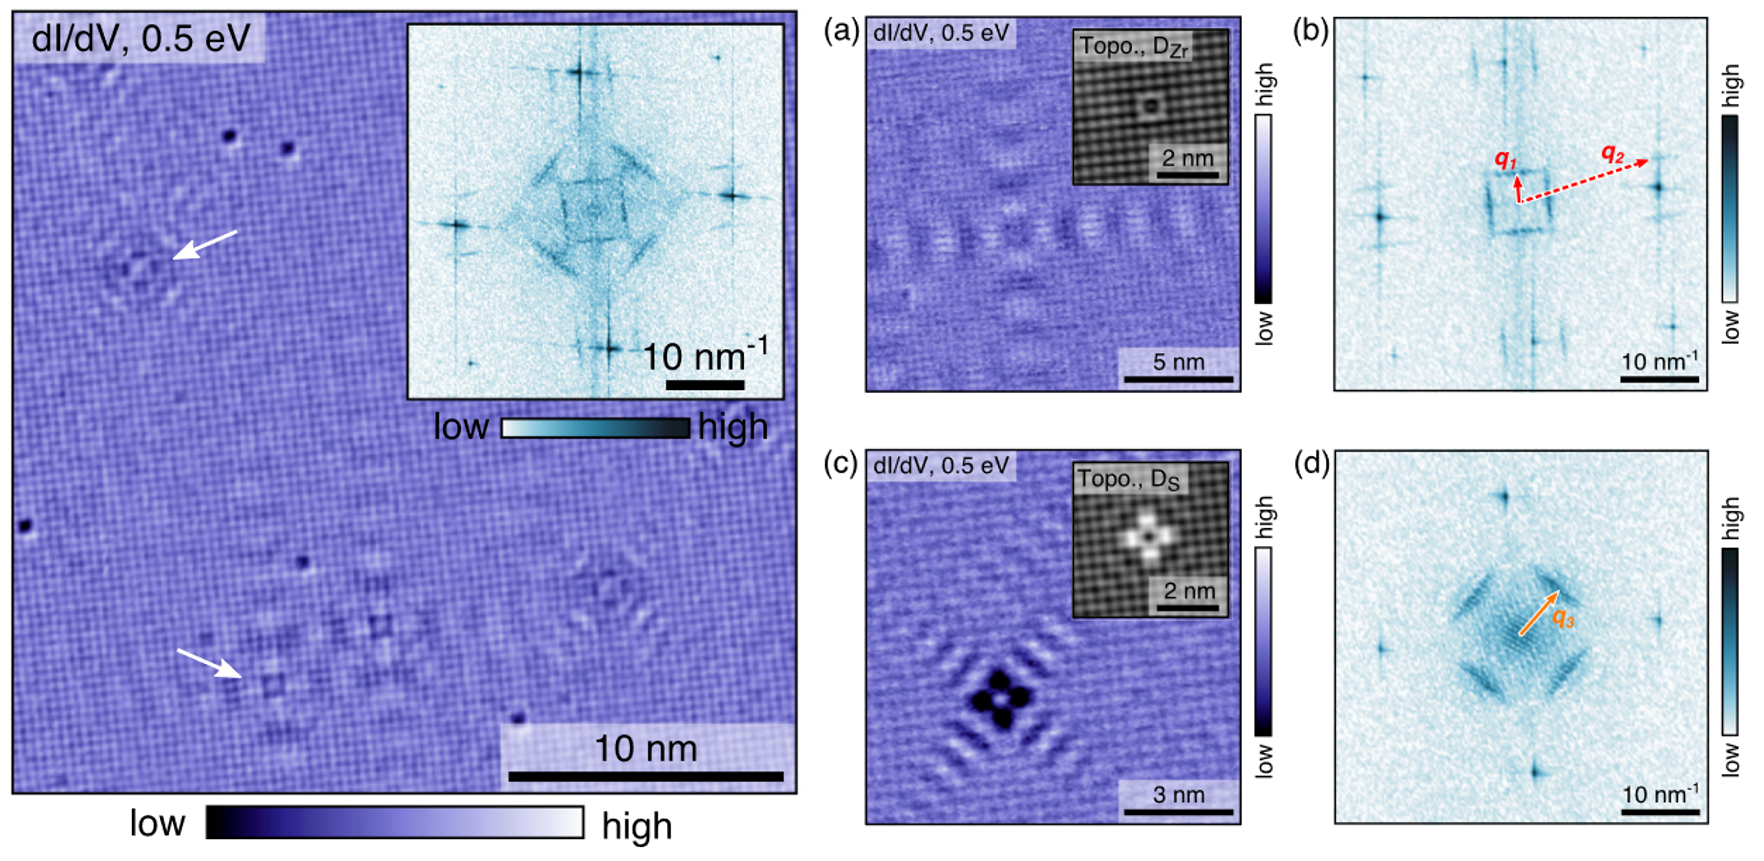
\includegraphics[width= \textwidth]{ZrSiS.png} 
	\centering
	\caption{}
	\label{fig:ch6_ZrSiS}
\end{figure}
%todo: add citations to corresponding literatures 

It is therefore preferred, if we can reconstruct the contribution of each individual type of defect from a big grid map that includes multiple types of defects; this is called the demixing problem.  

We now use our synthetic data to better illustrate the demixing problem. We simulate 2 \ac{QPI} patterns from 2 distinct defects with kernel choices A1 and A2 as shown in Fig. \ref{fig:ch6_demix} c) and d); We then define their activation maps X1 and X2 in d) and g). By summing up the convolutions between 2 kernels and their corresponding activation maps, we can obtain an observation Y in a). We express the above observation generation process as:

\begin{equation}
	Y = A1 * X1 + A2 * X2 + \beta, 
\end{equation}
where $\beta$ is the added noise determined by a pre-defined signal-to-noise ratio.

The demixing problem is the inverse of the observation generation process: given the observation 
Y, our goal is to reconstruct A1, A2, and their corresponding activation maps. This means that in reciprocal space, rather than working with entangled and less informative data like (b), we can recover disentangled QPI patterns from individual defect types, as shown in (e) and (h), which are also free from speckles. Lastly, we extend the above formulation with multiple types of different defects, then at arbitrary energy $\omega$, we have: 

\begin{equation}
	\label{eq:demixing}
	Y_{\omega} = \sum_d ( A_{d,{\omega}} * X_d) + \beta. 
\end{equation} 

\begin{figure}
	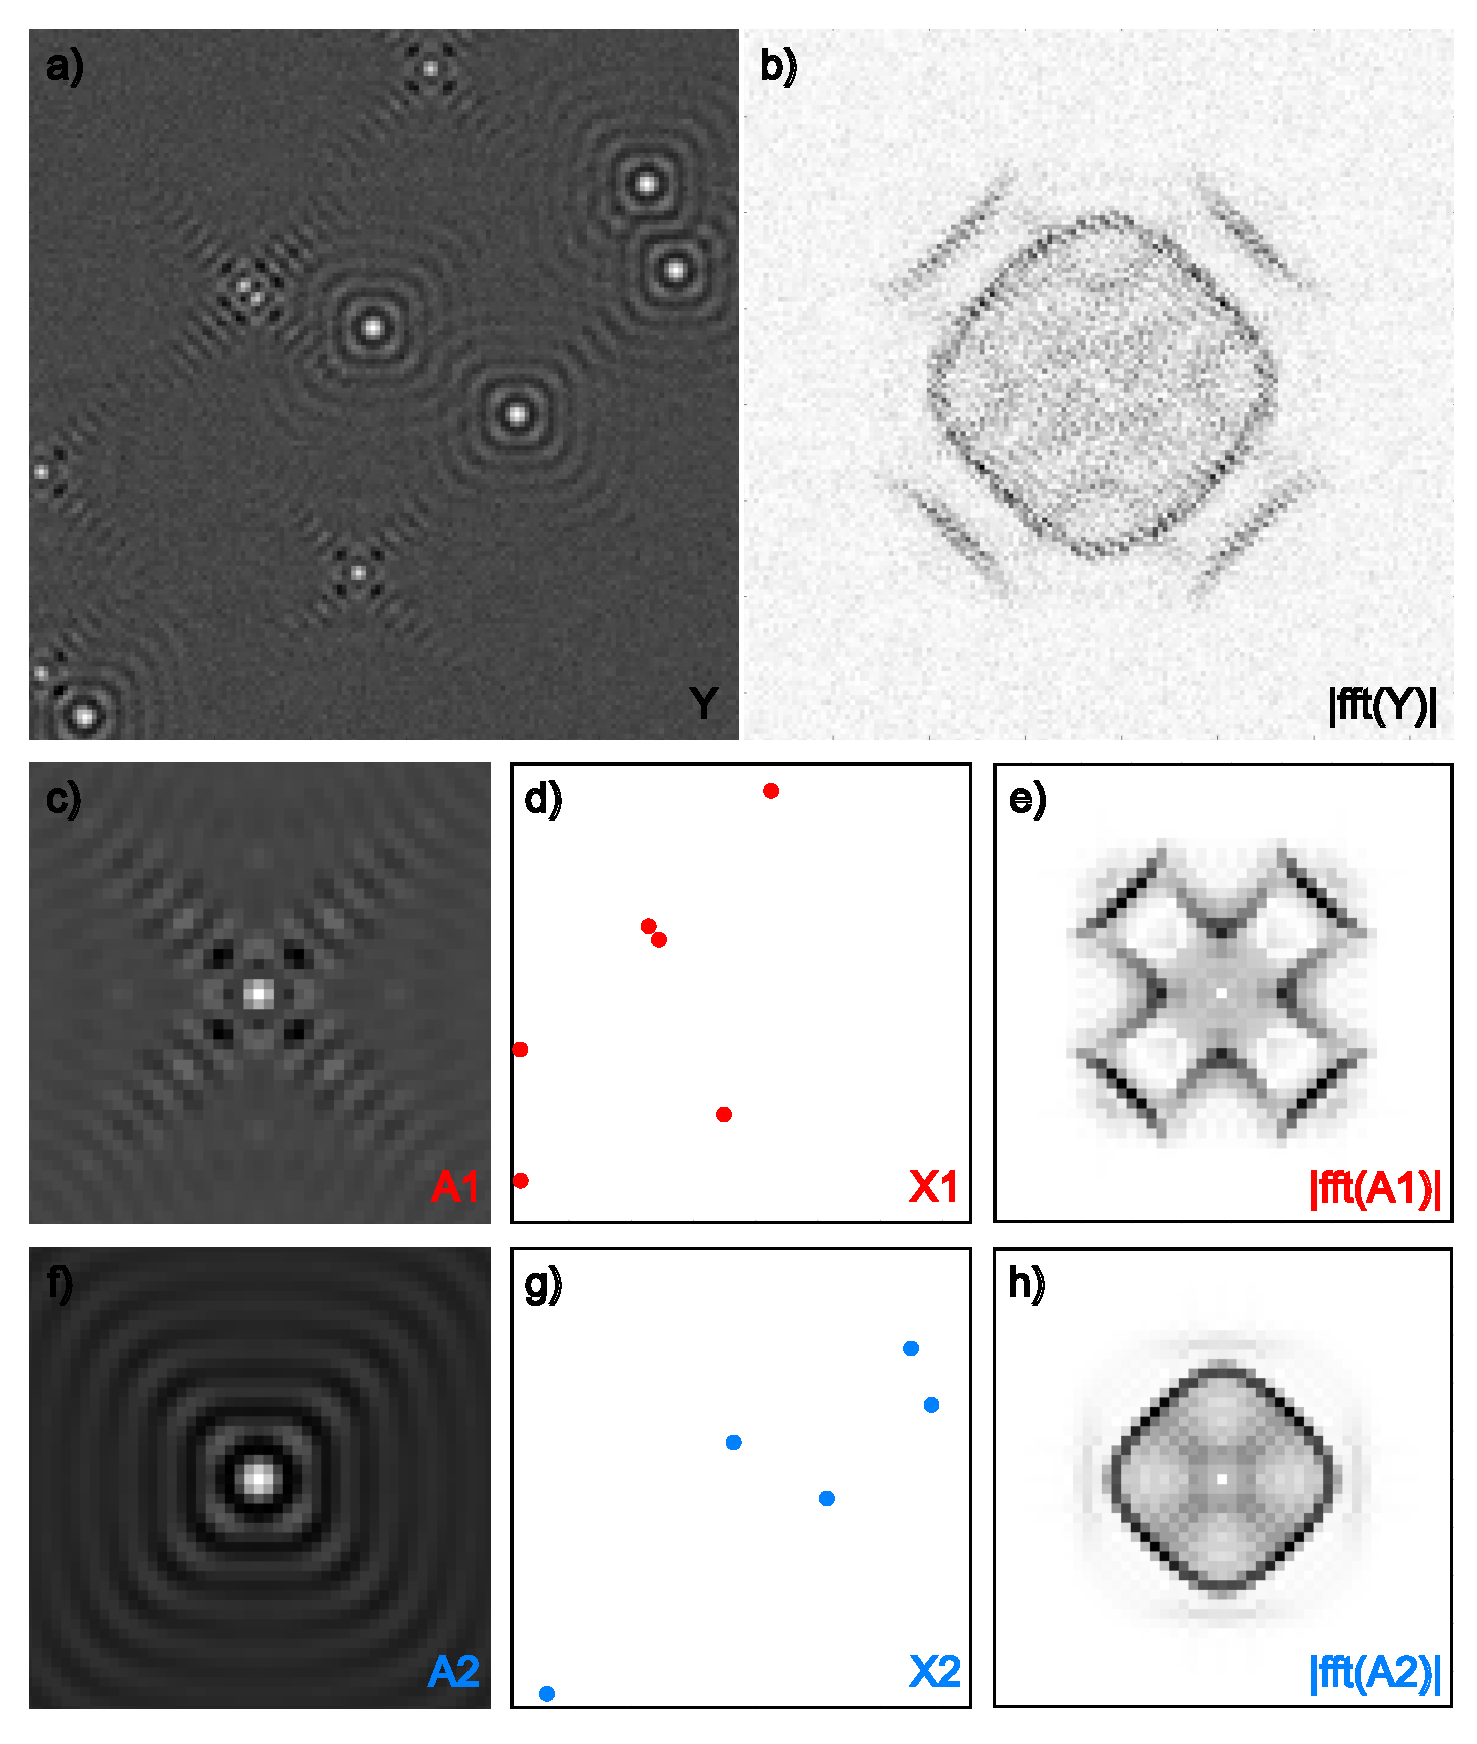
\includegraphics[width= \textwidth]{Ch6_demixing.pdf} 
	\centering
	\caption{}
	\label{fig:ch6_demix}
\end{figure}




\section{A convolutional model of STM}
A convolutional model of STM interpret STM spectroscopy measurement as the convolution of the features sourced from defects and their corresponding activation. The first convolutional model of STM was raised by Cheung et al \cite{cheungDictionaryLearningFouriertransform2020}; As shown in Figure \ref{fig:ch6_conv} a), an STM observation Y is the convolution of a kernel $A_0$ and its corresponding activation $X_0$. we extend the convolutional model to multi-type defect case, as hinted in Figure \ref{fig:ch6_demix}, we now have multiple kernels $A_d$ with different sizes and their corresponding activation map $X_d$. This is exactly what we formulated in the demixing problem with Equation \ref{eq:demixing}:

\begin{equation}
	Y_{\omega} = \sum_d ( A_{d,{\omega}} * X_d) + \beta,
\end{equation}
\noindent where observation $Y_{\omega} \in \mathbb{R}^{n_1 \times n_2}$ is the \ac{LDOS} slice of size at bias energy $V_{bias} = \omega$, $A_{d,{\omega}} \in \mathbb{R}^{m_1^d \times m_2^d}$ is the kernel correspond to the $d^{th}$ defect, $X_{d} \in \mathbb{R}^{n_1 \times n_2}$ is the activation map of the $d^{th}$ defect, and $\beta \in \mathbb{R}^{n_1 \times n_2}$ is the additive noise. 

\noindent It is worth noting that the kernels could vary in different energy slices, as the energy dispersion of QPI patterns are normally non-trivial, and the noise level may also vary at different energies. On the other hand, the activation map should stay the same across all energies, as the defect location should be fixed. The task of recovering all $A_d$ and $X_d$ given $Y$ can be formulated as a \ac{MC-SBD} problem. 
 
\begin{figure}
	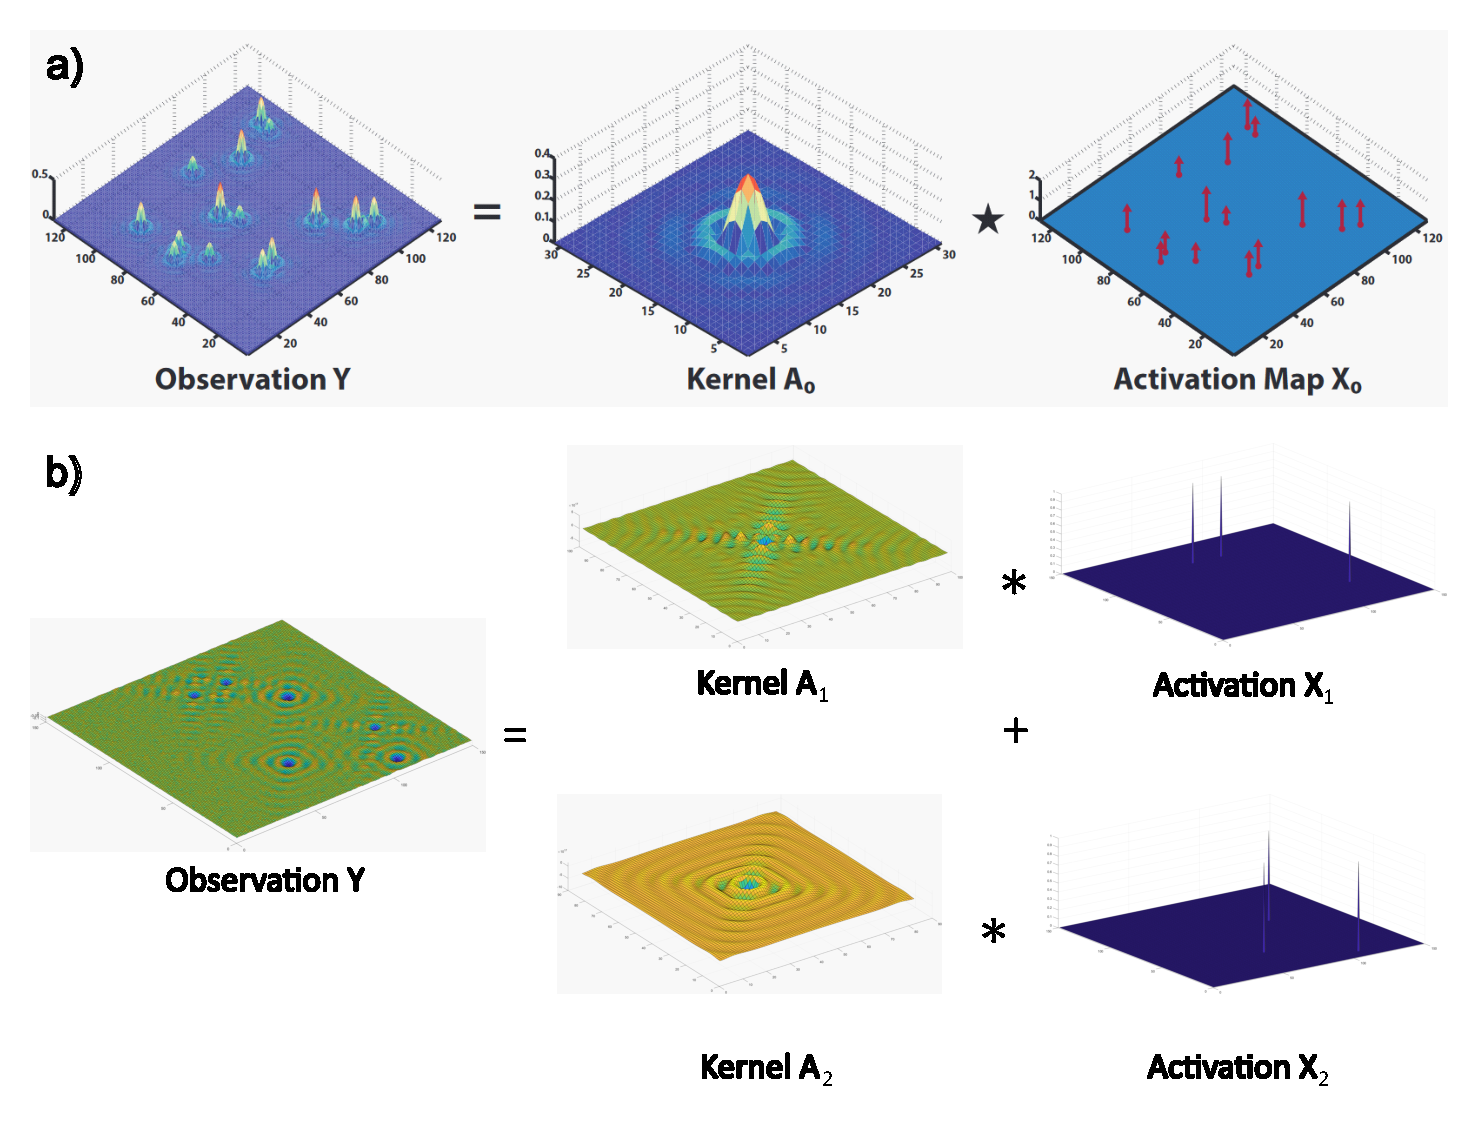
\includegraphics[width= \textwidth]{convolutional_model.pdf} 
	\centering
	\caption{Convolutional model of STM grid spectroscopy. a) Single defect convolutional model, introduced by Cheung et al to solve Sparse Blind Deconvolution(SBD) problem.\cite{cheungDictionaryLearningFouriertransform2020}. b) Multi-defect convolutional model, used to address \ac{MC-SBD} problem.}
	\label{fig:ch6_conv}
\end{figure}


\subsection{formulation of Multi-Channel Sparse Blind Deconvolution problem}
To understand the \ac{MC-SBD} problem, we need to first formulate its single-channel case --  the \ac{SBD} problem. Recall we can express the observed \ac{LDOS} $\delta\rho$ as the convolution between an individual QPI $\delta\rho_0$ and its defect location function $D(\mathbf{x})$ as: 
\begin{equation}
	\delta \rho(\mathbf{x}, \omega) = (\delta \rho_0 *D)(\mathbf{x}, \omega).
\end{equation}

\begin{figure}
	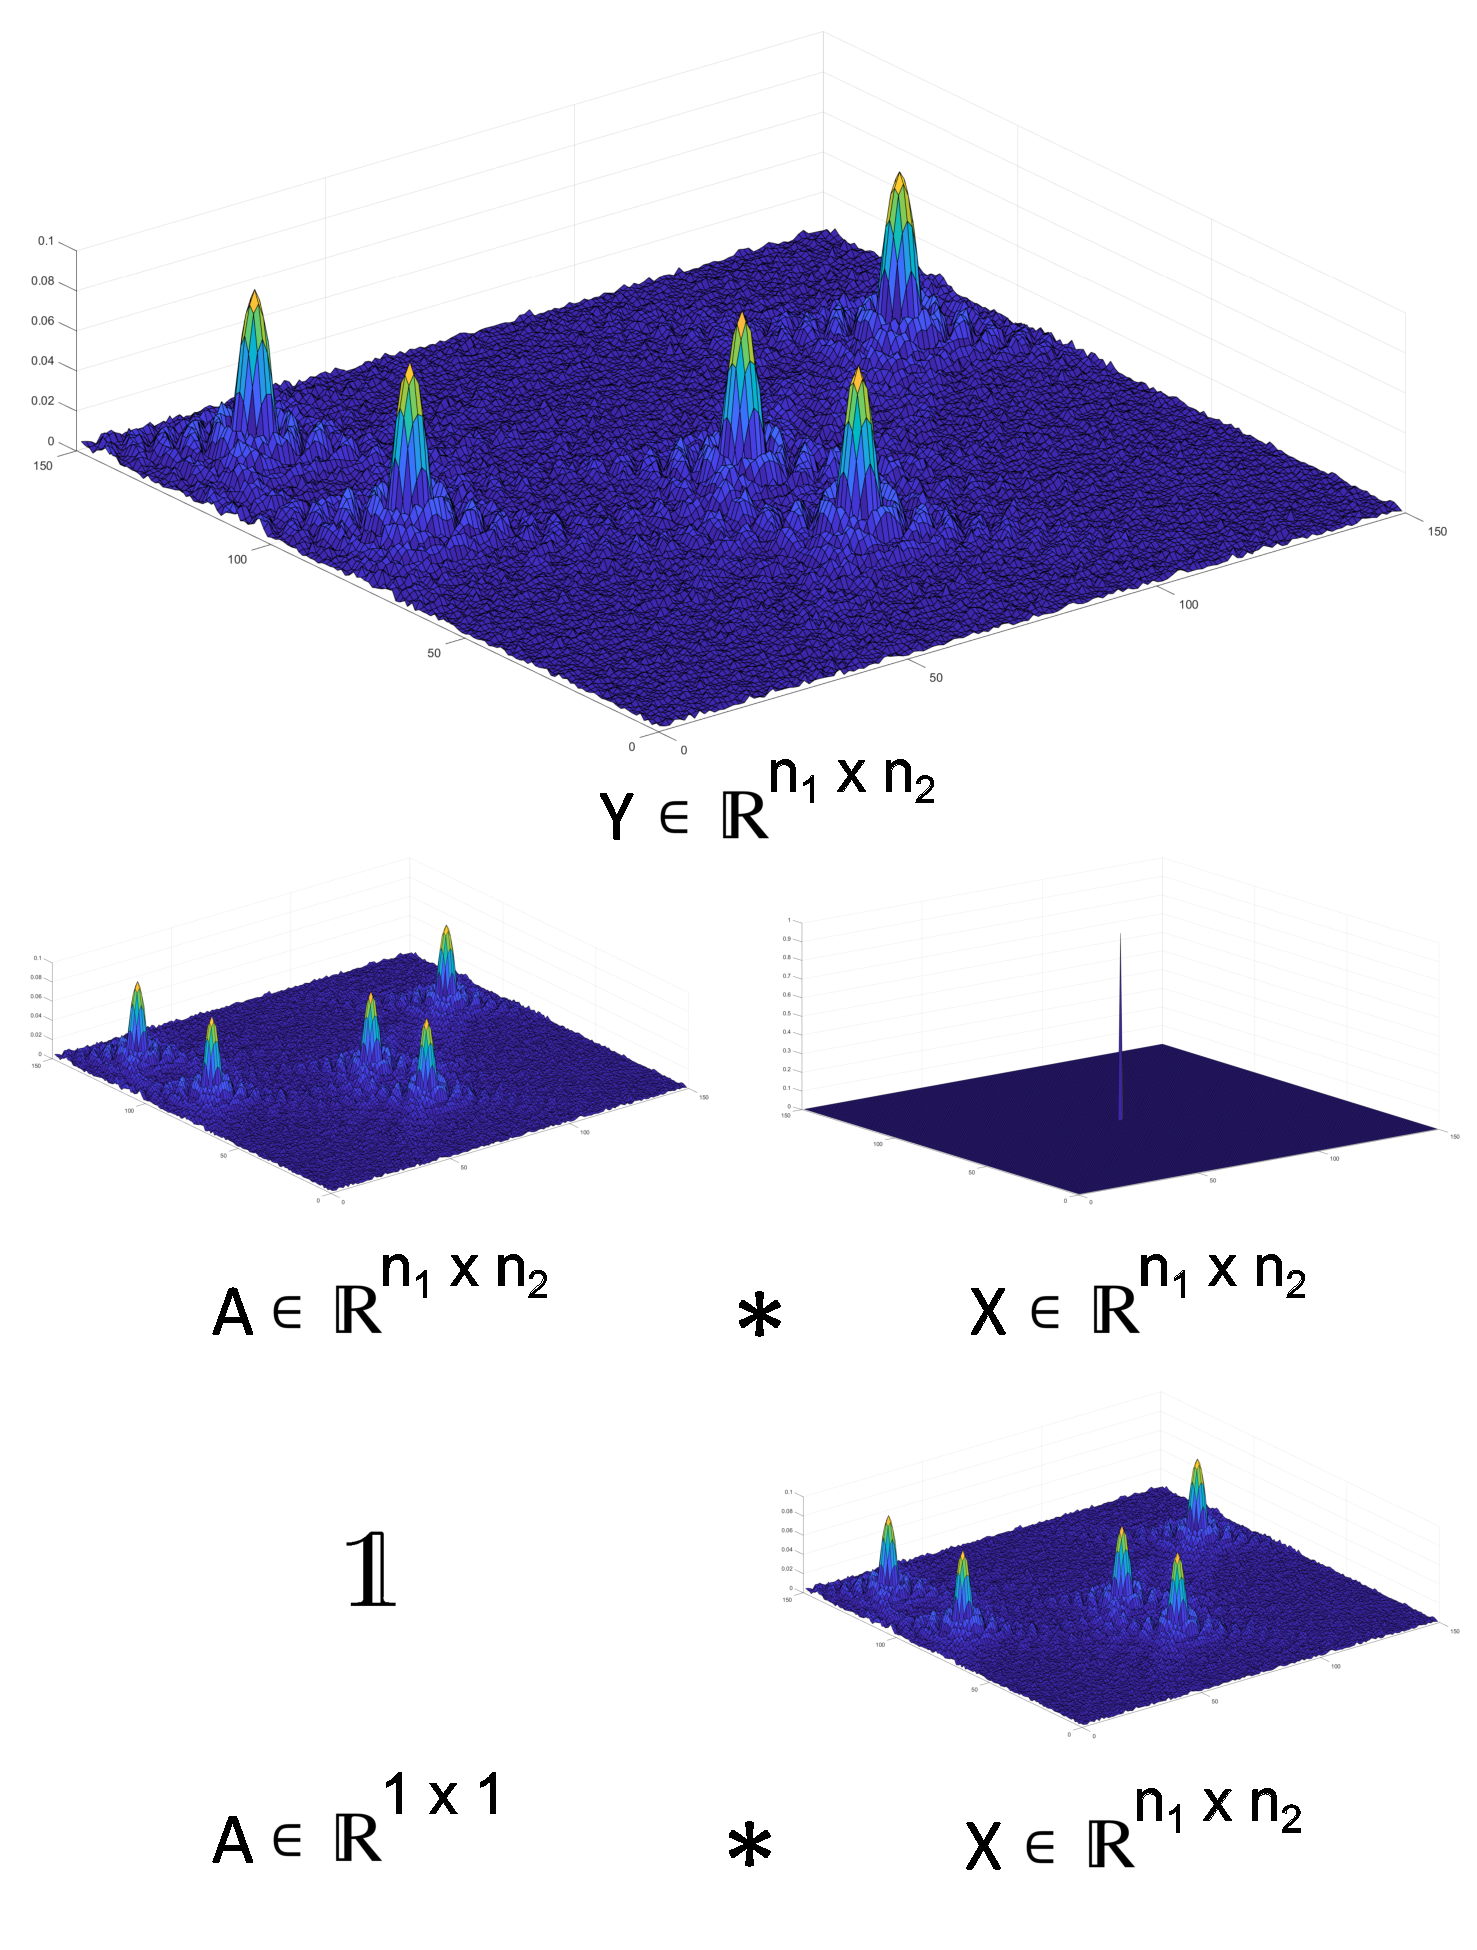
\includegraphics[width= \textwidth]{associativity.pdf} 
	\centering
	\caption{An extreme case illustrating associative symmetry of convolution. For any observation Y, there will always be two convolutions: one being we have a trivial activation, and all information is stored in the kernel with the same size as Y; The other is when we have a trivial scalar activation, and all information is stored in the activation}
	\label{fig:ch6_assoc}
\end{figure}

\noindent If we know the individual QPI pattern $\delta\rho_0$, and given the observed $\delta\rho$, we can inverse the convolution and get the defect location function $D(x)$; This is a deconvolution process. However, when $\delta\rho_0$ is unknown, it becomes a bilinear inverse problem known as \ac{BD}. However, as you may see, this is an ill-posed question, as there are many degenerate pairs of $(\delta\rho_0, D(\mathbf{x}))$ that could reconstruct the same observation. The reason behind these degeneracy is that the convolution is symmetric over several operations: 
\begin{itemize}
	\item \textbf{Translation Symmetry}: We obtain the same observation if we shift the kernel and activation map by an in-plane vector $\vec{\Delta}$ in the opposite direction. That is, given a translation operator $\operatorname{T}[f,\vec{\Delta}] \equiv f(\vec{x}+\vec{\Delta})$, we have:  
	\begin{equation}
		A_0 * X_0 = T[A_0,\vec{\Delta}] * T[X_0, -\vec{\Delta}].
	\end{equation}
	\item \textbf{Associative Symmetry}: Convolution operation is associative, meaning $(f * g) * h = f * (g *h)$, this has two implications, one is we have scaling symmetry: given $g = \alpha$, where $\alpha$ is a non-zero scalar, we have: 
	\begin{equation}
		A_0 * X_0 = (\frac{1}{\alpha})A_0*\alpha X_0.
	\end{equation}
	Another less trivial implication is we can have information leak between the kernel and the activation; That is, given $A_0 = A_0^L * A_0^R$ and $X_0= X_0^L * X_0^R$, where we express the kernel and the activation as convolutions, we have: 
	\begin{equation}
		A_0 * X_0 = (A_0^L * A_0^R * X_0^L) * X_0^R = A_0^L * (A_0^R * X_0^L * X_0^R).
	\end{equation}
	We can illustrate this with an extreme case shown in \ref{fig:ch6_assoc}. Given observation Y, two deconvolutional solutions are guaranteed by the associative symmetry, one is when the kernel resembles the observation and activation map is a delta function centered at the image origin, another is when all information leaked to the activation, and we are left with a trivial scalar kernel. While these extreme cases are not differentiable by the machine, they may seem absurd to us human; This is because we possess some intrinsic assumptions about the structure of both the kernel and the activation. By structuring our assumptions into rigorous formulations, we can indeed turn this ill-posed \ac{BD} problem well-posed. 
	
\end{itemize}



To break these symmetries and thus the corresponding degeneracy is crucial for a robust and reliable reconstruction. common approaches to break the symmetries including setting constrains to the manifold and introducing asymmetries to the cost function. For example,  enforcing A to stay in a hypersphere manifold $S = \{A \in \mathbb{R}^{m_1 \times m_2}: \vert\vert A \vert \vert_{F}= 1\}$, we can break the scaling symmetry except for the case when $\alpha = -1$. Additionally, the translation symmetry can be addressed by realizing the decaying nature for a QPI pattern, that is, the intensity near the edge of a kernel should approach zero; However, this restrain is weaker for kernels with larger size; this is illustrated in Figure.\ref{fig:ch6_t&s}, a) is the ground truth QPI pattern, it satisfy the constrain we set as the edge intensity naturally approaches zero due to the decay. We can then pad around a) with zeros to get a new kernel like b), note that this will still satisfy our constrains; We can pad it differently as shown in c) and d), thus recreating the degeneracy due to the translation symmetry. For this reason, we will see later that setting a proper spatial kernel size is crucial for our algorithm. 

Introducing asymmetries in the cost function is another important implementation, it is hard to visualize with problems in higher dimensions, we thus illustrate this with an example in 3D shown in Figure \ref{fig:ch6_reg}. Given potential energy $E_1 = sin(3x)\cdot cos(3x)$ with multiple local minimums, we can introducing a radial term $\lambda_r(x^2 + y^2$) to bias the local minimums closer to the origin, we can further tune the strength of the radial bias with $\lambda_r$ and set up a favorable energy landscape. This additional bias term is referred as a regularizar in the field of optimization, by assigning a proper regularizar to the cost function, we can turn the initially non-convex landscape to a more convex landscape, allowing a more stable and robust optimization. In our case, we will address the non-trivial associative symmetry by introducing a sparsity regularizar. 

\begin{figure}
	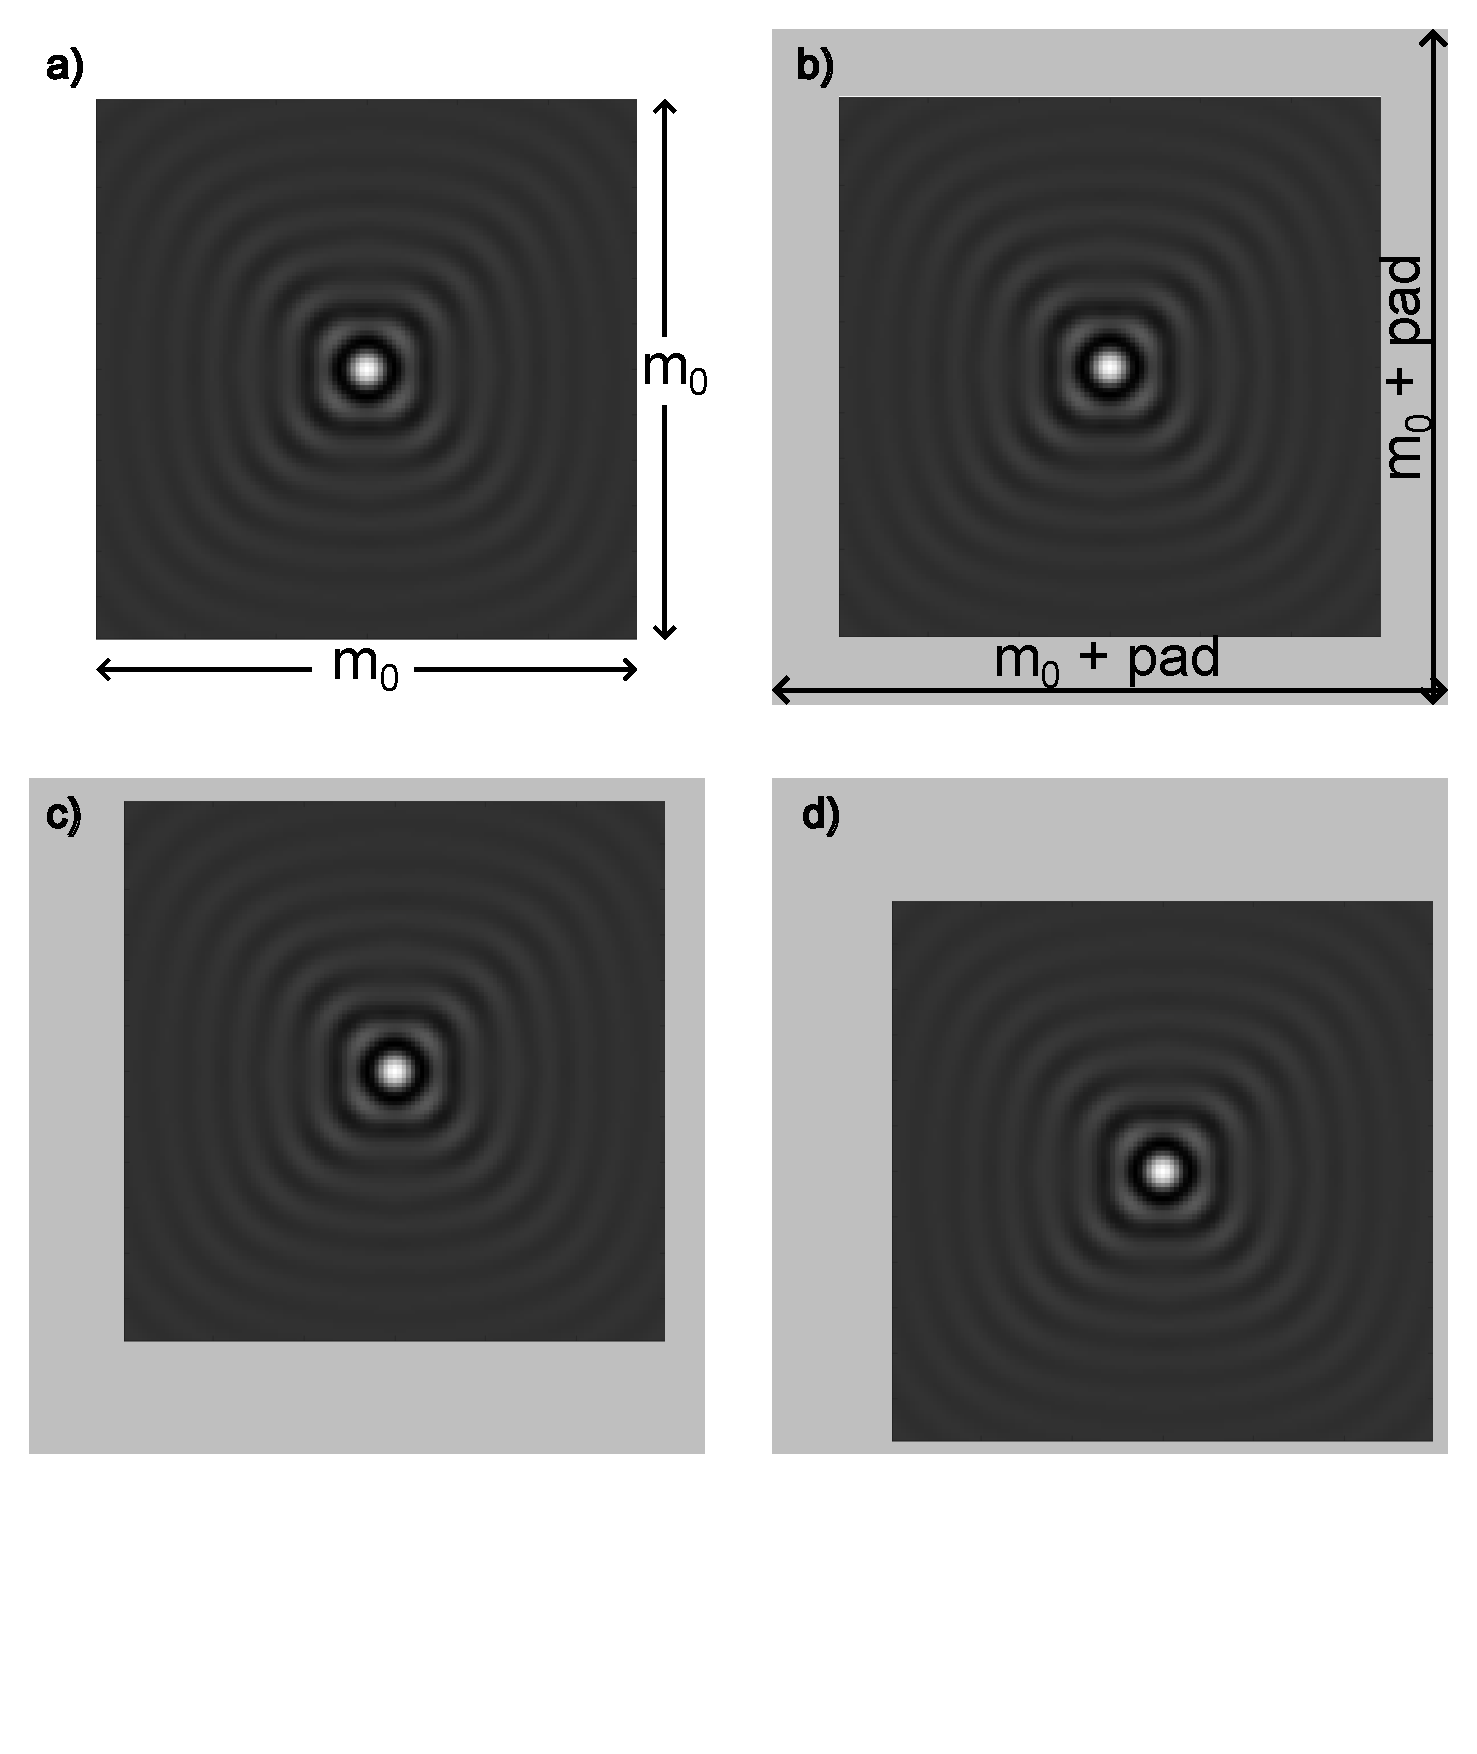
\includegraphics[width= \textwidth]{truncate and shift.pdf} 
	\centering
	\caption{Degeneracy caused by large kernel size. Given the ground truth QPI pattern (a) of size $m_0 \times m_0$, which naturally decays to near-zero intensity at the edges (or to the noise level in practical cases), this represents the ideal kernel we aim to reconstruct. However, ambiguity arises when constructing alternative kernels, such as in (b)–(d), by padding the ideal kernel with noise while preserving the vanishing edge condition. As the kernel size increases, the space of such degenerate solutions also grows, making the inverse problem increasingly ill-posed.}
	\label{fig:ch6_t&s}
\end{figure}

\begin{figure}
	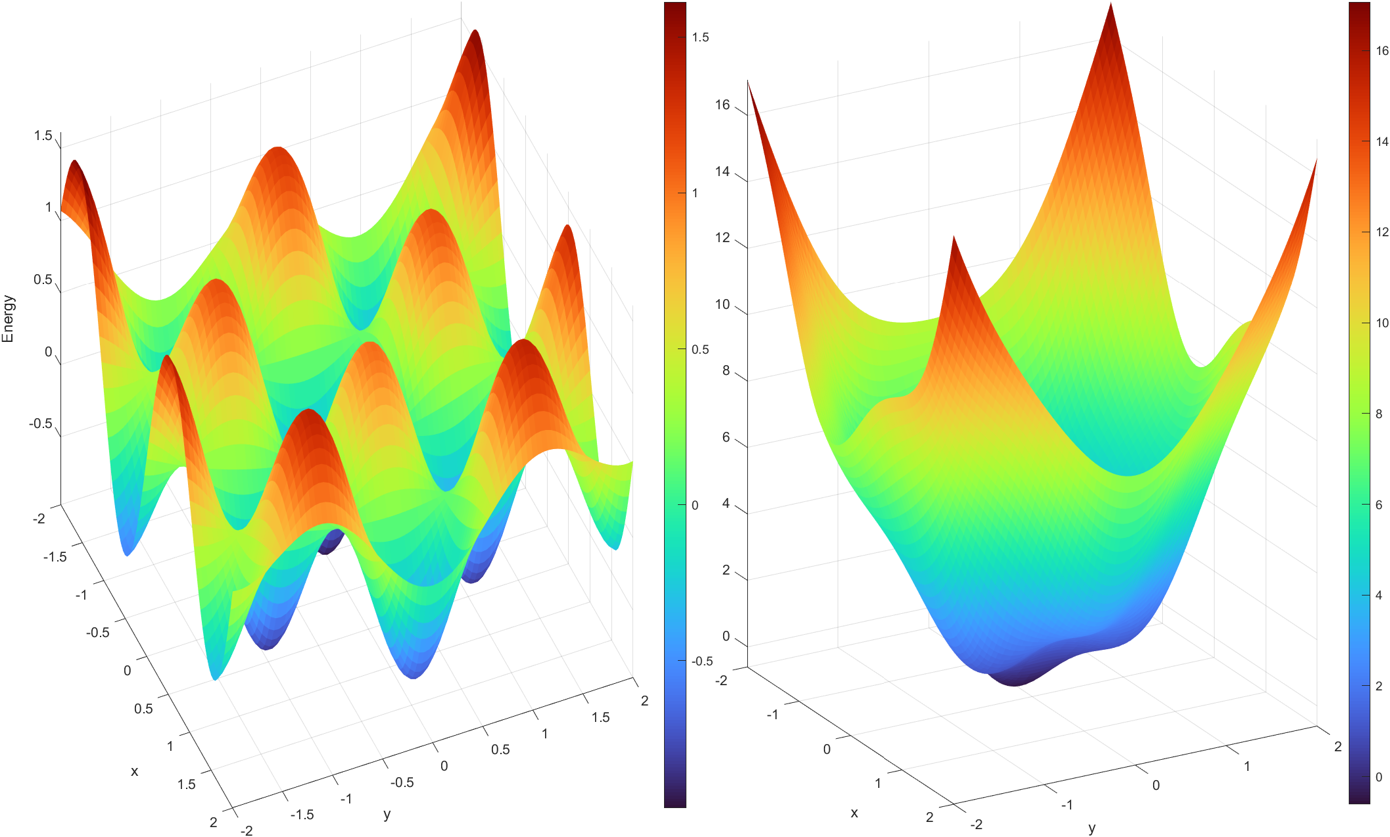
\includegraphics[width= \textwidth]{energy_reg.png} 
	\centering
	\caption{A low-dimension schematic showing how regularizar can make an initial non-convex problem convex. Left is the energy landscape created by $E_1 = sin(3x)\cdot cos(3x)$, this landscape is periodic in both spatial directions; Minimizing the energy is non-convex and ill-posed. However, if we add a regularizer $\phi_r \equiv \lambda_r(x^2 + y^2)$; with proper $\lambda$, this radial term will make $E_2 = E_1 + \phi_r$ convex. Right is an example of $E_2$ when we take $\lambda=2$.}
	\label{fig:ch6_reg}
\end{figure}

\subsubsection{The role of sparsity}
The sparsity regularizar acts on the activation map, by definition, an activation map $X_0$ is sparse when most of its entries are zero. Intuitively, we can define the regularizar to be proportional to $\left\lVert X\right\rVert_0$ -- X's $l_0$-norm, which is equal to the number of non-zero elements in $X$; However, $l_0$-norm is discrete and makes the cost function lost its continuity, which is harmful for the optimization process. We therefore replace $\left\lVert X\right\rVert_0$ with the $l_1$-norm $\left\lVert X\right\rVert_1 = \sum_{i=1}^{n}\vert x_i \vert$. We thus want to find $A_0$ and $X_0$ that minimize cost function $\phi_{\lambda}$:
\begin{equation}
	\phi_{\lambda} = \frac{1}{2}\left\lVert A_0 * X_0 - Y \right\rVert^2_F + \lambda \cdot \left\lVert X\right\rVert_1;
\end{equation}
\noindent The first term represent the data fidelity, where $\left\lVert \cdot\right\rVert_F$ represent the \textit{Frobenius norm}: 
\[
\left\lVert A \right\rVert_F = \sqrt{ \sum_{i=1}^{m} \sum_{j=1}^{n} |a_{ij}|^2 };
\] 
\noindent And $\lambda$ is a tunable parameter that we can set to vary the strength of the regularizer; Although bigger $\lambda$ normally results in a more convex problem, it can also overweight the data fidelity term and thus makes the result undesirable, a suitable range of $\lambda$ can be explored and tested in the practical runs. It is also worth noticing that in practice, even with an ideal $\lambda$, there may still be local minimums, making the problem non-convex globally, therefore, a good initial guess is usually required, especially for more challenging cases with multiple defects. 

We should discuss the validity of the sparse requirement for activation map. Recall that in our case, activation map $X$ represent the defect location map $D$, and the non-zero entries in the defect location map indicate the presence of a defect in the scan. Thus, lower defect concentration justifies the sparse requirement better. We can estimate a quantitative line of defect concentration where the sparse requirement could breakdown: Typically, a grid map takes a spatial linear resolution of 2-3 pixels per unit cell, for a square grid with the same linear resolution on each side, we have $\approx 10$ sampling points for a given unit cell. Note that the sparse requirement state that number of defects $N_d$ being much smaller than the sampling point $N_s = n_1 \times n_2$, say $N_d < \frac{N_s}{100}$, we get a cutoff defect concentration of $N_d^{cutoff} \approx 0.1$ per unit cell. This is a large defect concentration, moreover, this is the requirement not for the total defect concentration, but for a single type of defect; Thus, in most cases, it is safe to assume we satisfy the sparse requirement. However, dense defect cases can still break the assumption, and we will see in the later chapter that the algorithm's performance drops in the dense defect regime. 

\subsubsection{Complexity in Multi-Channel SBD}
We use the sparse nature of activation map to turn the bilinear Blind-Deconvolution problem into a better-posed Sparse Blind-Deconvolution problem. However, to address demixing problem, we need to encode multiple defect types into the algorithm formulation, this introduces extra level of complexity. 

First, multiple channels increases the dimension of the manifold, thus making the optimization process more computationally expensive. Another key source of complexity is the additional symmetries introduced with multi-channel, we illustrate these additional symmetries with a simplified 2-defect-type case, with the ground truth kernel and activation indicated with a superscript $gt$: 
\begin{equation*}
	Y = A_1^{gt}*X_1^{gt} + A_2^{gt}*X_2^{gt}
\end{equation*} 

\begin{itemize}
	\item \textbf{Linear Mixing Equivalence}: This equivalence roots from the distributive rule of the convolution: $(f_1+f_2)*g = f_1*g + f_2*g$. Given: 
	\begin{align*}
		A_1 &= aA_1^{gt}+bA_2^{gt}, \\
		A_2 &= cA_1^{gt}+dA_2^{gt}, \\
		X_1 &= a'X_1^{gt}+b'X_2^{gt}, \\
		X_2 &= c'X_1^{gt}+d'X_2^{gt}; \\
	\end{align*}
	We have: 
	\begin{align*}
		A_1*X_1 +A_2*X_2= (aa'+cc') A_1^{gt}*X_1^{gt}+ (bb'+dd')A_2^{gt}*X_2^{gt} \\+ (ab'+cd') A_1^{gt}*X_2^{gt} +(ba'+dc') A_2^{gt}*X_1^{gt},
	\end{align*}
	To ensure $A_1*X_1 +A_2*X_2 = A_1^{gt}*X_1^{gt} + A_2^{gt}*X_2^{gt}$, we meed to consider two cases, the easier case is when we have two very distinctive ground truth kernels and the off-diagonal terms are linearly-independent from the diagonal terms. Thus, we want to eliminate the $A_1^{gt}*X_2^{gt}$ and $A_2^{gt}*X_1^{gt}$ terms, and we need to satisfy:
	 \begin{align*}
	 	ab'+cd'&= ba' + dc' = 0, \\
	 	aa'+cc'&= bb' + dd' = 1; \\
	 \end{align*}
	 With 4 equations and 8 unknowns, we are left with 4 degrees of freedom within the degeneracy space. Note that this is with 2 types of defects, with n types of defects, the degeneracy space will expand with n square. In the case of similar ground truth kernels, we might have cross-talks between the off-diagonal terms and diagonal terms; This leaves us with a even larger degeneracy space. 
\end{itemize}

In real STM studies, materials usually present more types of defects. As illustrated in Figure \ref{fig:ch6_defect} a), it is an STM topography taken on ZrSiTe, there are 4 distinct types of defects circled in red, moreover, we have the same type of defect but rotated 90 degrees circled in yellow. It is not uncommon to see rotated defects, as defect formation follows the lattice symmetry; The rotation of same type of defect can be better illustrated in PtSn$_4$ as shown in b), where 4 croissant defects at 4 orientations are circled in yellow. In \ac{MC-SBD}, each orientations of the croissant defects will be treated as a new type of defect, therefore, even with only 1 type of defect, we might need to use multiple kernels; This further shows the challenging nature of the problem, as well as the necessity to extend the single defect \ac{SBD} algorithm to \ac{MC-SBD}.

\begin{figure}
	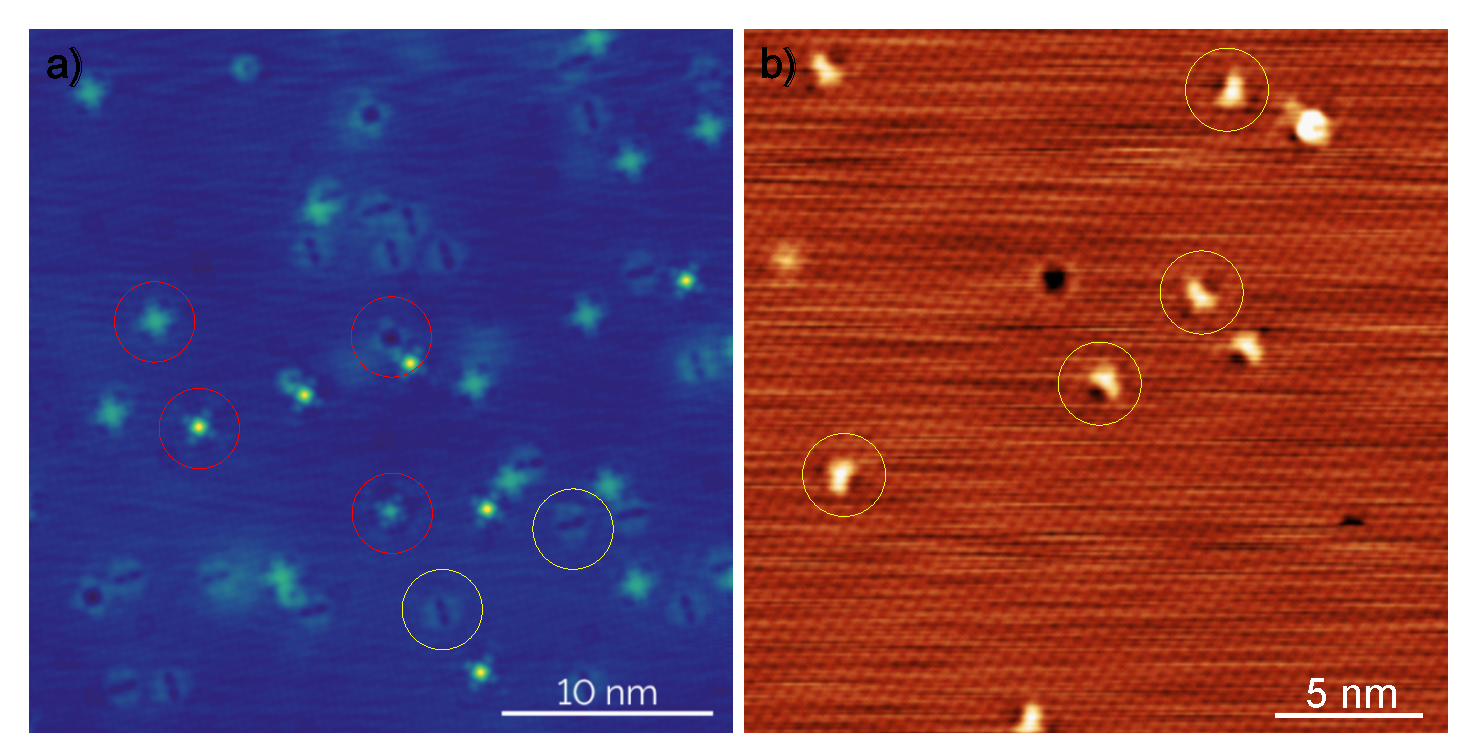
\includegraphics[width= \textwidth]{defect_types.pdf} 
	\centering
	\caption{}
	\label{fig:ch6_defect}
\end{figure}
\pagebreak
\section{A Multi-Channel Sparse Blind Deconvolution approach to STM}

In this chapter, we will introduce our approach to address the \ac{MC-SBD} problem. We will first analyze the bi-linear nature of \ac{MC-SBD}, and overview the possible methods that address it. We then briefly introduce the Riemannian Trust Region method (RTRM), a direct non-convex optimization algorithm that addresses the \ac{SBD} problem. Finally, we present our algorithm which extends \ac{RTRM} to multiple-channel cases. 

\ac{MC-SBD}, also known as the joint sparse blind deconvolution/demixing problem is a bi-linear problem, that is, the observed signal is modeled as a convolution (or equivalent linear operation) between pairs of two unknowns—and this operation is linear in each variable when the other is fixed, but not jointly linear. Bi-linear problems can be solved by either a lifted method or a direct method. A lifted method can formulate the initial bi-linear mapping of two unknowns to a linear mapping of a single unknown, by defining a one-to-one mapping from two unknowns to the targeted unknown. For example, given observation $y = \mathbb{A}(x,h)$, where $x \in \mathbb{R}^n$ and $h \in \mathbb{R}^m$ are two inputs we try to recover. We can define an outer product $X = xh^T\in \mathbb{R}^{n\times m}$, and rewrite observation $y = \mathbb{A'}(X)$. In the case of convolution, $\mathbb{A'}$ is the Lifted circular convolution operator. A lifted problem can be solved analytically, and since we are dealing with only one subspace defined by $X$, by assigning constraints on $(x,h)$,  $X$ usually present some internal structures, and we are left with a fully convex problem; thus, the convergence to global minimum can usually be proven, this is also known as the recovery guarantee. For example, Flinth et al. show that, given both inputs are sparse, they can achieve high probability recovery by lifting the \ac{MC-SBD} problem and applying a hierarchical sparsity framework[tocite]. 

However, in real cases, it is rare to find both inputs sparse. Moreover, the lifting method is normally computationally inefficient, as the dimension of output space is the product of two separate inputs, it expands quickly with higher input dimensions, making it unfavorable for larger size problems like the QPI-STM recovery, note that it is even more expensive in the multi-channel case, as now the dimension of output space is not only product of two input space but product of $2 \cdot types$ input spaces. On the contrary, a direct method updates one input while assuming the other one is fixed, the optimization space of the problem thus grows linearly with the input dimension. The trade-off is that with direct methods, recovery guarantee is hard to obtain, instead, local minimal recovery can be guaranteed with careful algorithm design. Local convergence can be combined with an initial guess that is close to the global minimum; this recipe of combining a good initial guess and an algorithm with strong guarantees of local convergence usually leads to good recovery. 

Our algorithm is a direct method that follows the above recipe, it utilizes Riemannian Trust Region Method(RTRM) to provide local convergence. Standard Trust Region Method is a second-order method that guarantees local minimum recovery, as long as the objective(ie, the cost function $\phi$) has no degenerate stationary points, that is, the Hessian $\Delta^2\phi$ has no zero eigenvalues. This ensures a sufficiently curved optimization landscape for the algorithm to make consistent progress. Moreover, compared to first-order methods based on gradient descent, Trust Region Methods has significantly faster convergences and a better overall tail convergence when the iterates are close to local minima. 

\ac{RTRM} is first raised by Absil et al. in 2007 as the extension of Trust Region Methods on a Riemannian sub-manifold, embedded in Euclidean spaces. This is advantageous since enforcing our manifold to follow certain geometry, for example in our case, we enforce the kernel to live on a hypersphere $S$ defined by Equation \ref{hypersphere}, which removes the scaling symmetry we discussed. As a result, the \ac{RTRM} provides strong guarantees that a local minimum of the objective be attained over S. We now present the \ac{RTRM} algorithm used by Cheung et al. \cite{cheungDictionaryLearningFouriertransform2020} that addresses \ac{SBD} problem; we then build on it and present our \ac{MC-SBD} algorithm. 

\subsection{SBD algorithm}
Recall we have the objective function $\phi_{\lambda}$: 
\begin{equation}
	\phi_{\lambda} = \frac{1}{2}\left\lVert A_0 * X_0 - Y \right\rVert^2_F + \lambda \cdot  \left\lVert X\right\rVert_1,
\end{equation}
since \ac{RTRM} is a second-order method, we need to make make our objective function smooth, more particular, we need to smooth the sparse regularizer. This can be achieved by approximate the $l_1-norm$ by $r_{\mu}(X)$:
\begin{equation}
	r_{\mu}(X) \equiv \sum_{i,j} \mu^2(\sqrt{1+\mu^{-2}\cdot X_{i,j}}-1), 
\end{equation}
this is called a pseudo-Huber regularizer, in the limit of $\mu -> 0$, the regularizar resembles $l_1-norm$, in our case, we choose $\mu = 10^{-6}$. 

To adopt a direct method as we discussed, we will updates each input to minimize the objective function while assuming the other input fixed. We now solve: 
\begin{equation}
	\label{sbdalgorithm}
	(\hat{A}, \hat{X}) \leftarrow \min_{{A} \in {S}} \left\{ 
	\phi_{\lambda}({A}) \equiv \min_{X} \left[ 
	\phi_{\lambda}({A}, {X}) \equiv \frac{1}{2} \left\| {A} * {X} - {Y} \right\|_F^2 
	+ \lambda \cdot r_{\mu}({X}) 
	\right] 
	\right\}.
\end{equation}
This updating algorithm consists of an inner and an outer solver. The inner solver: $X \leftarrow \mathbf{XSolve}(A, \lambda)$, that is, obtaining $\hat{X}$ that minimizes $\phi_{\lambda}(A,X)$ using \ac{RTRM}. The outer solver: $A \leftarrow \mathbf{ASolve}(A, \hat{X}, \lambda)$, updating $A$ that minimizes $\phi_{\lambda}(A,X)$ using \ac{RTRM}. Since $\mathbf{XSolve}$ is an intermediate step, for $i^{th}$ iteration, we can simply write the process as: $(A^{i+1}, X^{i+1}) \leftarrow \mathbf{ASolve}(A^{i}, X^{i}, \lambda; Y,(m_1,m_2))$, where $(m_1,m_2)$ is the predefined kernel size. Or for a complete process of in total n such loops, we write $(A, X) \leftarrow \mathbf{ASolve}^n(A, X, \lambda; Y,(m_1,m_2))$

We can then write the Complete SBD-STM procedure: 

\begin{algorithm}
	\label{SBDalgo}
	\caption{Complete SBD-STM Procedure}
	\textbf{Input:}
	\begin{itemize}
		\item Observation $Y \in \mathbb{R}^{n_1 \times n_2 \times s}$,
		\item Kernel size $(m_1, m_2)$,
		\item Initial $\lambda_0 \geq 0$, decay rate $\alpha \in [0,1)$, and final $\lambda_{\text{end}} \geq 0$.
	\end{itemize}
	
	\textbf{Phase I:}
	\begin{enumerate}
		\item Randomly initialize: $A^{(0)} \in S = \mathbb{S}^{m_1 \times m_2 \times s}$.
		\item $A_\star^{(0)} \leftarrow \texttt{ASolve}^N(A^{(0)}, \lambda_0, loop)$.
	\end{enumerate}
	
	\textbf{Phase II:}
	\begin{enumerate}
		\item Lifting: Get $A^{(1)} \in S' = \mathbb{S}^{m_1' \times m_2' \times s}$ by zero-padding the edges of $A_\star^{(0)}$ with a border of width $\left\lfloor \frac{m_1}{2} \right\rfloor$.
		\item Set $\lambda_1 = \lambda_0$.
		\item Refinement: \textbf{Repeat} for $k = 1, 2, \dots$ \textbf{until} $\lambda_k \leq \lambda_{\text{end}}$,
		\begin{enumerate}
			\item[(a)] $A_\star^{(k)} \leftarrow \texttt{ASolve}^N(A^{(k)}, \lambda_k)$,
			\item[(b)] \textbf{Centering}:
			\begin{enumerate}
				\item[i.] Find the size $m_1 \times m_2$ submatrix of $A_\star^{(k)}$ that maximizes the Frobenius (square) norm across all $m_1 \times m_2$ submatrices.
				\item[ii.] Get $A^{(k+1)}$ by shifting $A_\star^{(k)}$ so that the chosen $m_1 \times m_2$ restriction is in the center, removing and zero-padding entries as needed.
				\item[iii.] Normalize $A^{(k+1)}$ so it lies in $S'$.
			\end{enumerate}
			\item[(c)] Set $\lambda_{k+1} = \alpha \lambda_k$.
		\end{enumerate}
	\end{enumerate}
	
	\textbf{Output:}
	\begin{itemize}
		\item Extract $\hat{A} \in S$ by extracting the restriction of the final $A^{(k+1)}$ to the center $m_1 \times m_2$ window.
		\item Find the corresponding activation map $\hat{X} \in \mathbb{R}^{n_1 \times n_2}$ by solving $\min_{X} \psi_{\lambda_k}(\hat{A}, X)$.
	\end{itemize}
\end{algorithm}

The kernel $A^{(0)}$ is first randomly initialized and normalized, it is then fed into two phases sequentially. Both phases utilize the same core algorithm $\mathbf{ASolve}$ as described above. Phase I aims to obtain a primary kernel $A^{(0)}_*$ given $\lambda_0$. Phase II serves as a refinement that increases the recovery quality by applying a stricter sparsity regularizer $\lambda_{k} > \lambda_0$, as well as addresses the degeneracy brought by the translation symmetry formulated in Equation \ref{translational_symm}. The latter is achieved by applying a so-called shift-truncate method, as illustrated in Figure. \ref{fig:ch6_phase2}. This method lifts the primary kernel $A^{(0)}_*$ by zero padding its edge with zeros to get a padded kernel with bigger size $(m_1',m_2')$, the padded kernel is then fed into $\mathbf{ASolve}$ with stricter $\lambda_{k}$ and get $A^{(k)}_*$ as shown in b). The Frobenius square norms are calculated on all the possible submatrices with size $(m_1,m_2)$ within $A^{(k)}_*$. An example of the submatrix window is illustrated in red square in b), and we can generate a heat map as shown in c), with each pixel in the heat map corresponding to a submatrix. The algorithm then finds the submatrix that maximizes the norm, which corresponds to the red cross in c), and we then truncate according to this submatrix and normalize it to get $A^{(k+1)}$. 

Using the Frobenius square norm score in the shift-truncate method is common practice and works well in most cases. However, it fails in more complicated situations, especially when we have other features in the padded kernel, this is illustrated in Figure. \ref{fig:ch6_phase2mod}, given primary kernel $A^{(0)}_*$, we pad it and apply $\mathbf{ASolve}$ to get $A^{(1)}_*$. The Frobenius square norm score is shown in c) and by picking the maximum, we get e), which resembles the primary kernel. This issue is mainly due to faint features around the primary feature. We can improve this algorithm by applying a radial decay term $\eta_d(r) = e^{-lnd \cdot r}$ to the Frobenius square norm, where r is the normalized distance from the submatrix window center, and d is the tunable decay factor. This biases the center features and is consistent with the decaying nature of the QPI patterns. With this decay term (d=2) applied, we obtain a heat map $S'$ as shown in d), and a truncated kernel $A^{(1)'}$ in f) has the primary more centered compared to e). For convenience, unless otherwise mentioned, all phase II that we introduced later will be using the center-biased Frobenius square norm. 

\begin{figure}
	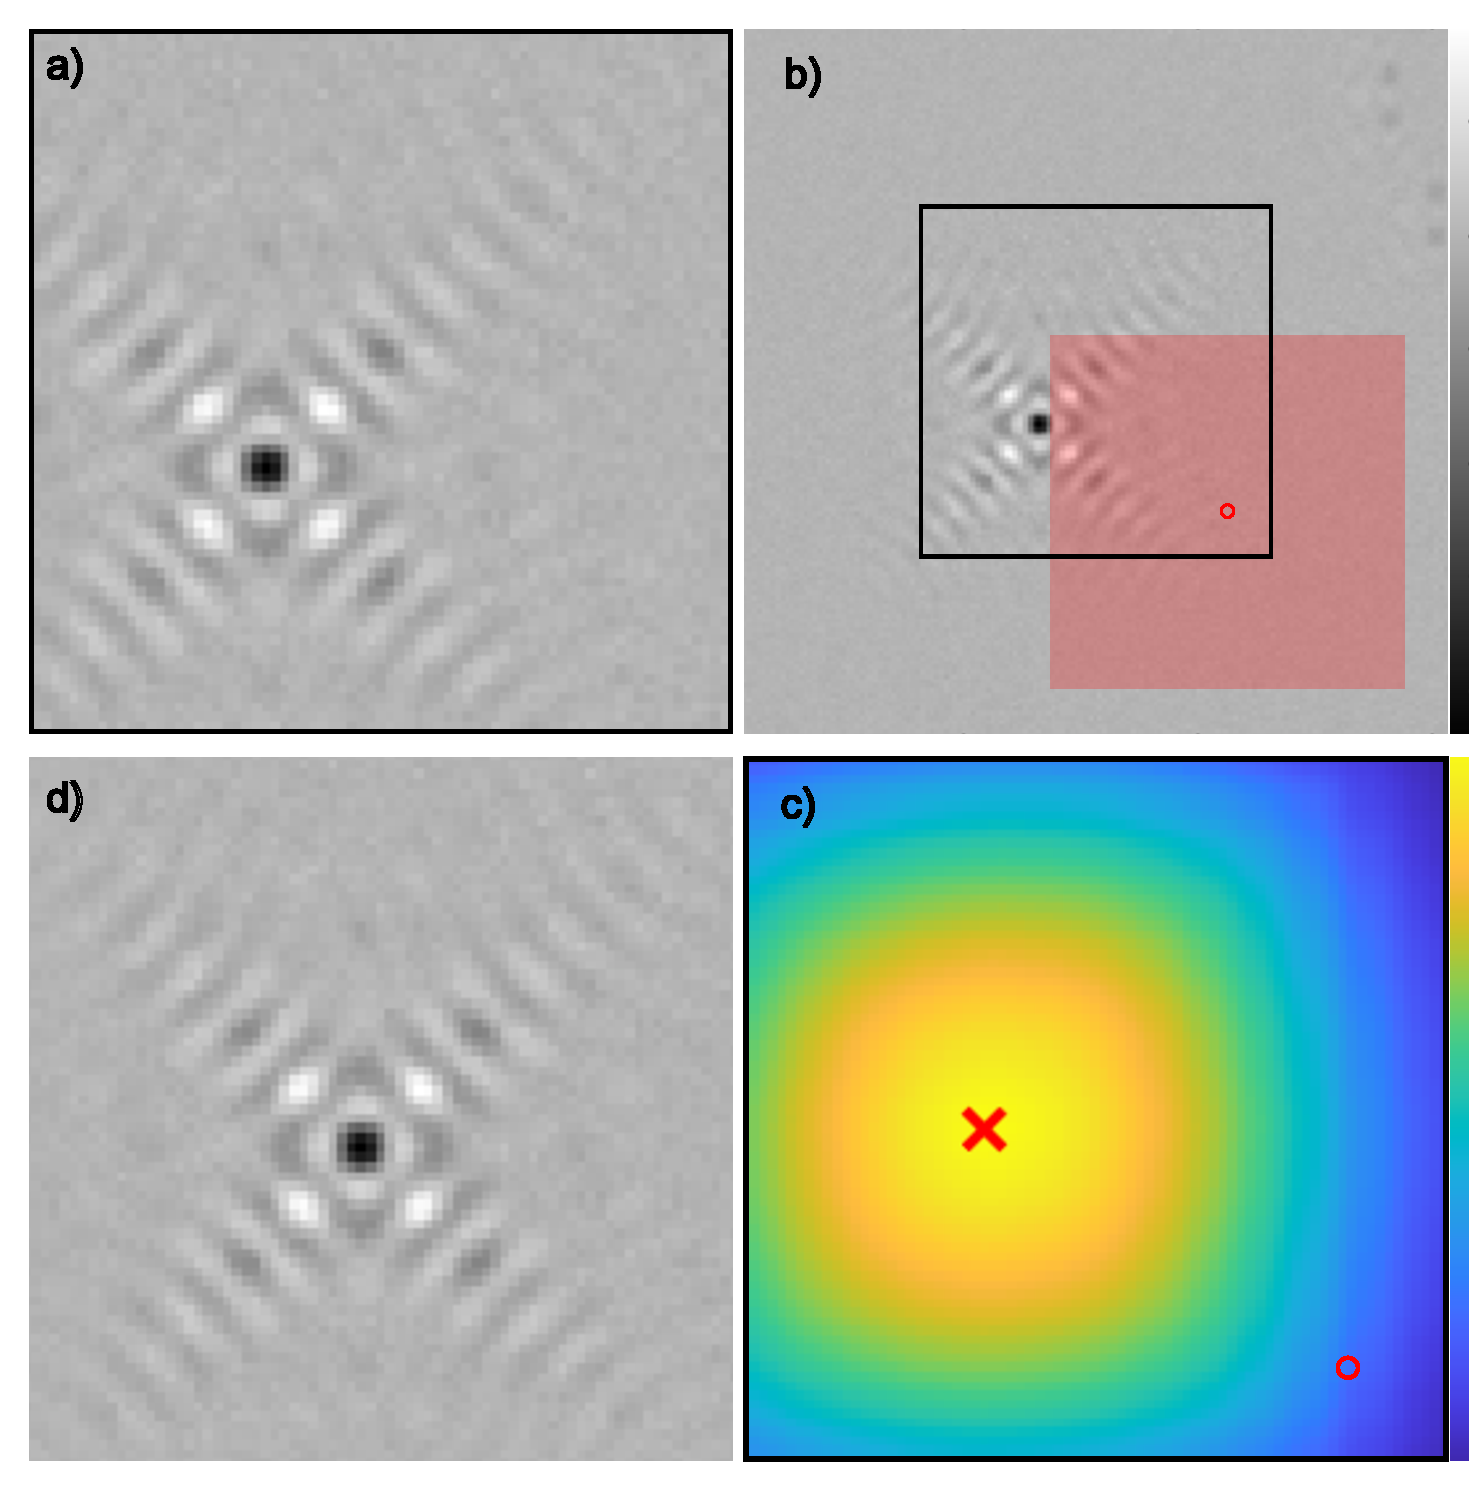
\includegraphics[width= \textwidth]{phase2old.pdf}
	\centering
	\caption{}
	\label{fig:ch6_phase2}
\end{figure}


\begin{figure}
	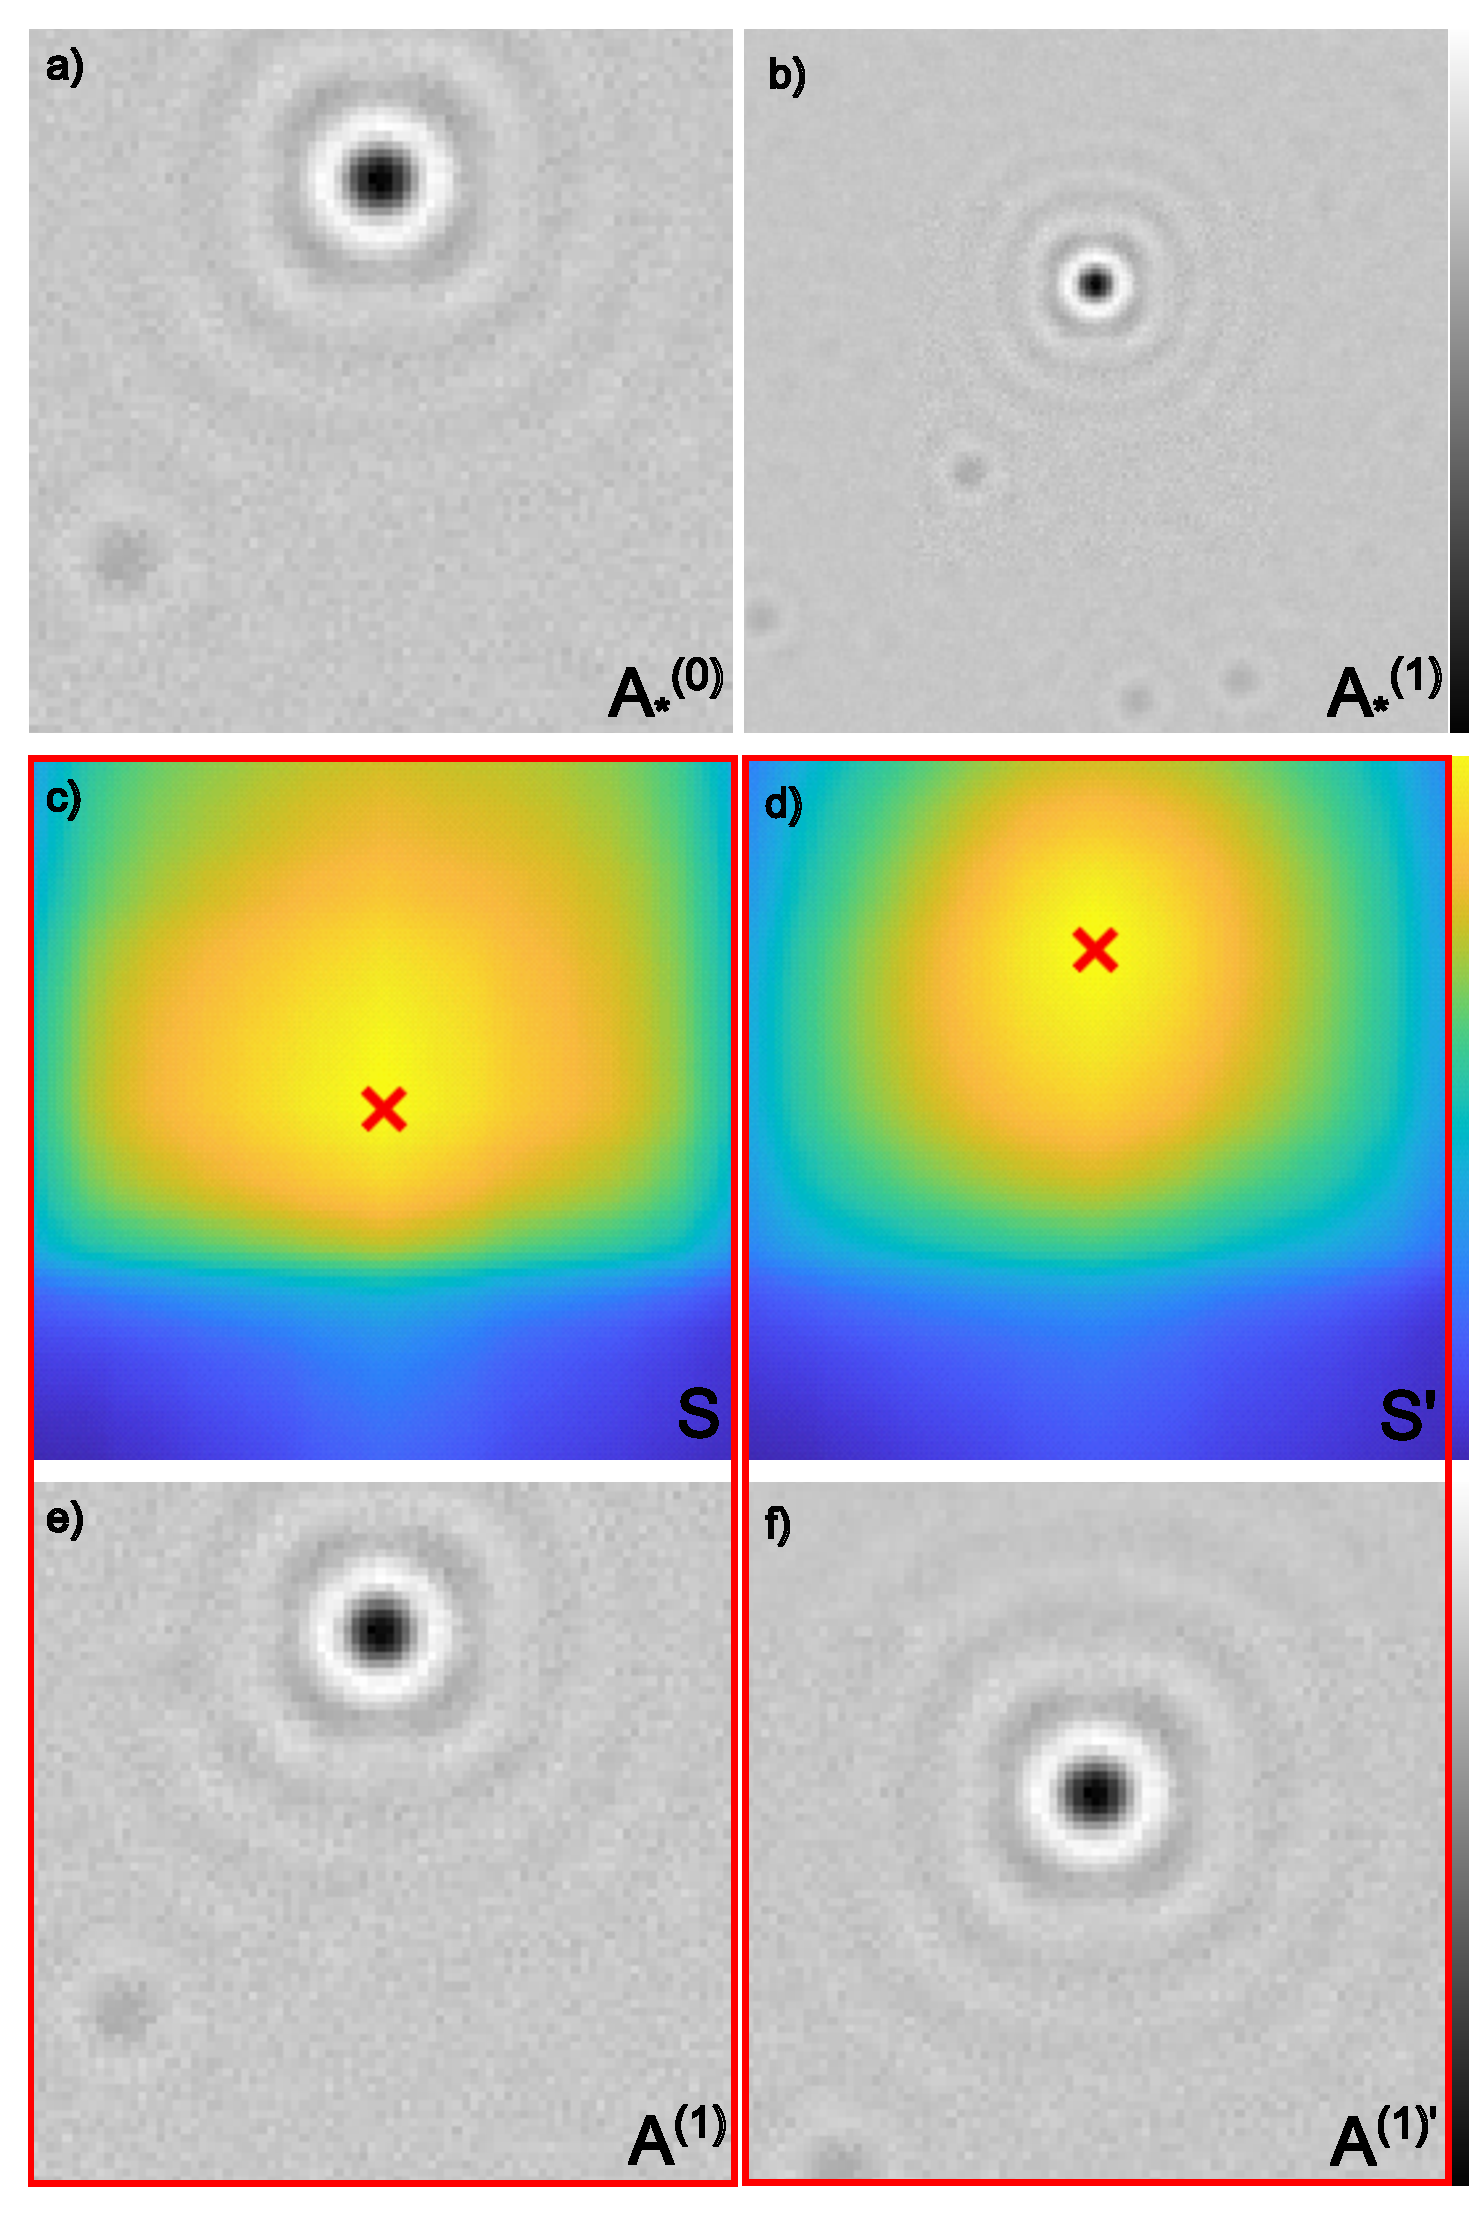
\includegraphics[width= \textwidth]{phase2mod.pdf}
	\centering
	\caption{}
	\label{fig:ch6_phase2mod}
\end{figure}


\subsection{MC-SBD algorithm}
We first establish some intuition about the multi-channel blind deconvolution process. Consider a generation process of the observation $Y$: 
\begin{equation}
	\label{eq:dec}
	Y = \sum_{i}^{s} A_i^{gt} * X_i^{gt} + noise, 
\end{equation}
\noindent where the superscript $gt$ indicate the ground truth. \ac{MC-SBD} aims to deconvolute multiple kernel-activation pairs given observation $Y$, such that $A_i=A_i^{gt}$ and $X_i = X_i^{gt}$, for all types $i \in [1,2,...,s]$. We can rewrite Equation \ref{eq:dec} as: 
\begin{align}
	Y &= \sum_{i}^{s} Y_i^{gt} + noise,\\ 
	Y_i^{gt} &= A_i^{gt} * X_i^{gt}.
\end{align}
\noindent This hints at the two separate operations in the data generation process: convolution and composition. Therefore, our \ac{MC-SBD} follows the reverse order: we first decompose the observation into kernel-specific components and then deconvolute each component into its kernel and activation. 

Due to the two-stage nature of the process, we adopt a hierarchical direct treatment across both the intra-type and the inter-type levels. At the intra-type level, when updating a specific kernel $A_j$, we hold its corresponding activation $X_j$ fixed -- a strategy inherited from the single-type \ac{SBD} algorithm. At the inter-type level, when handling the $j$-th type, we treat all $Y_i, i\neq j$ as fixed. 

This hierarchical approach enables isolated analysis for each type’s recovery:
\begin{align}
	Y_j &= Y - [\sum_{i\neq j}Y_i + noise],\\
	A_j * X_j &= Y - [\sum_{i\neq j}Y_i + noise].
\end{align} 
\noindent We can then write $Y_i = Y_i^{gt}- Y_i^{residual}$ and substitute the observation with \ref{eq:dec}. Then we have:
\begin{align}
	A_j * X_j &= \sum_{i}^{s} Y_i^{gt} + noise' - [\sum_{i\neq j}(Y_i^{gt}- Y_i^{residual}) + noise],\\ \label{eq:622}
	A_j * X_j &= Y_j^{gt}+ \sum_{i\neq j}Y_i^{residual} + noise = Y_j,
\end{align} 

\noindent The combined noise terms are absorbed into a single term. Equation \ref{eq:622} now resembles a single blind deconvolution problem, which can be addressed using the \ac{SBD} algorithm.

Smaller $Y_i^{residual}$ values for all $i \neq j$ lead to better-posed subproblems for each type. Consequently, when updating with the \ac{SBD} algorithm, we can produce a result $Y_j = A_j* X_j$ that is closer to the true component $Y_j^{gt}$. This motivates a loop structure in our algorithm: by updating one type (e.g. $j$), we reduce its residual $Y_j^{residual}$, which in turn helps improve the subsequent recovery of another type $i \neq j$. Through iterative refinement, given the local convergence guarantees provided by the \ac{RTRM} method, the residuals across all types could be gradually minimized, allowing the full reconstruction to converge towards the ground truth. However, this logic can break down in the early stages of optimization, where the residuals are large and noisy—making it difficult for the algorithm to enter a reliable refinement path. To address this challenge, we designed specific strategies that guide the optimization toward stability and correctness during these critical initial steps.

A complete description of the \ac{MC-SBD} algorithm is presented in Algorithm \ref{MTSBDalgo}; it preserves the two-phase structure from the original \ac{SBD} method. Apart from the loop structure discussed above, two important strategies are worth noting. 

First, The blending strategy is a dynamic weighting mechanism that constructs an effective observation for each kernel by combining the current residual with the global reconstruction: 
\begin{equation}
	Y_i = Y_{res} + \left(1-\frac{1}{\beta t+1}\right)A_i * X_i + \frac{1}{\beta t+1}Y_{sum},
\end{equation}
\noindent where $Y_{sum} = \sum_{j=1}^s A_j * X_j$ represents the sum of all convolution pairs, and the blending factor $\beta > 0$ controls the rate at which the influence of other components decreases over iterations.

This approach is particularly important in the early stages of decomposition, where the residuals are large and noisy. Without blending, directly updating each kernel-activation pair using such corrupted residuals can lead to poor local minima and error accumulation across iterations. By using a blending factor $\beta$ to control the mixing ratio over time, the algorithm initially relies more on the global structure to stabilize updates and gradually shifts toward using the true residual as the decomposition improves. This smooth transition prevents the algorithm from veering off due to early missteps and guides it toward more reliable solutions.

Another strategy is the variance-based update ordering, it prioritizes kernel updates according to the magnitude of their kernel variance, processing high-variance components first. This ordering is crucial because the residual is updated sequentially after each kernel is refined, meaning earlier updates have a greater influence on the remaining residual. By addressing the most dominant structures in the data first, the algorithm quickly reduces the residual and improves the signal quality for the weaker components updated later. This leads to better-conditioned subproblems throughout the iteration and helps avoid cumulative distortion that could arise from poor early updates to minor components.

\begin{algorithm}
	\label{MTSBDalgo}
	\caption{Multi-Type SBD-STM Procedure}
	\textbf{Input:}
	\begin{itemize}
		\item Observation $Y \in \mathbb{R}^{n_1 \times n_2}$,
		\item Kernel size list $k \in \mathbb{R}^{s \times 2}$ for $s$ kernels,
		\item Initial $\lambda_{1,i} \geq 0$, and final $\lambda_{2,i} > \lambda_{1,i}$, for $i=1,\dots,s$.
		\item Border padding $k_{plus} \in \mathbb{R}^{s \times 2}$.
		\item Faint factor $\beta > 0 $ for demixing.
	\end{itemize}
	
	\textbf{Phase I:}
	\begin{enumerate}
		\item Initialize kernels $A^{(0)}_i \in \mathbb{R}^{k_i}$ for $i=1,\dots,s$
		\item Initialize activation
		\item For each global iteration $t=1,\dots,T$:
		\begin{enumerate}
			\item Compute residual: $Y_{res} = Y - Y_{sum}$; $Y_{sum} = \sum_{j=1}^s A_j * X_j$
			\item For each kernel $i$ in descending order of variance:
			\begin{enumerate}
				\item Set up $Y_{i} = Y_{res} + (1-\frac{1}{\beta t+1})A_i * X_i + \frac{1}{\beta t+1}Y_{sum}$
				\item Update $(A_i, X_i) \leftarrow \texttt{ASolve}^N(Y_{i}, A_i, \lambda_{1,i})$
				\item Update residual: $Y_{res} = Y_{i} - A_i * X_i$
			\end{enumerate}
		\end{enumerate}
	\end{enumerate}
	
	\textbf{Phase II:}
	\begin{enumerate}
		\item Lifting: For each kernel $i$:
		\begin{enumerate}
			\item Create $A^{(1)}_i \in \mathbb{R}^{k_i + 2k_{plus}}$ by zero-padding $A^{(0)}_i$ around the edge. 
		\end{enumerate}
		\item For each refinement $r=1,\dots,R$:
		\begin{enumerate}
			\item For each kernel $i$ in order:
			\begin{enumerate}
				\item $\lambda_i = \lambda_{1,i} +\frac{r}{R}(\lambda_{2,i}- \lambda_{1,i})$
				\item Set up $Y_{i} = Y_{res} + A_i^{(r)} * X_i^{(r)}$
				\item Update $(A_i^{(r+1)}, X_i^{(r+1)}) \leftarrow \texttt{ASolve}^N(Y_{i},  A_i^{(r)}, \lambda_i)$
				\item \textbf{Centering}:
				\begin{enumerate}
					\item Calculate score $s(\tau)$, the center-biased Frobenius (square) norm on the submatrices with every possible shift $\tau$.
					\item Find shift $\tau^*$ maximizing $s(\tau)$
					\item Shift kernel by $\tau^*$ and activation map by $-\tau^*$
				\end{enumerate}
				\item Update residual: $Y_{res} = Y_{i} - A_i^{(r+1)} * X_i^{(r+1)}$
			\end{enumerate}
		\end{enumerate}
	\end{enumerate}
	
	\textbf{Output:}
	\begin{itemize}
		\item Final kernels $\hat{A}_i \in \mathbb{R}^{k_i}$ extracted from center of padded kernels
		\item Calculate activation maps $\hat{X}_i \in \mathbb{R}^{n_1 \times n_2}$ with \texttt{XSolve}
	\end{itemize}
\end{algorithm}


\section{Existing Algorithm}
\subsection{Shortcomings of existing algorithm}
\begin{itemize}
	\item 1. Their simulation data used truncated QPI pattern, not true to the real STM case. 
	\item 2. Too ideal to be useful in most cases,
\end{itemize}

Shortcoming in generating the observations. The purpose here is to simulate as close to experiment as possible to test and benchmark this method. 

I would like to elaborate on the truncation they made, they are given a simulation result, say a $256\times256\times41$ of $\delta\rho$ covering say 50 by 50 lattice from single defect at the center, without considering the noise level, the authors truncate the initial 50 by 50 lattice down to 19 by 19. In the generation of the observation, a parameter is set to be the ratio between the kernel size versus the window size, by setting this, they determined target size of the kernel in pixel, and then they can reshape the 19 by 19 lattice simulation into the target size. While one can argue that this process of truncating and reshape did not hinder the purpose of testing the SBD algorithm. It fails to simulate what happened in the experiment. Note that with this method, the boundary of the real-space QPI pattern is artificially set by the truncation.

Physically, the boundary of real-space QPI pattern is resulted from the interplay between the quasiparticle lifetime and the noise level, as kind of illustrated in Fig. \ref{fig:ch5_cutoff}; Thus, the kernel-window size ratio can be calculated after setting up the designed noise level at an energy slice, and due to this direct correlation, we argue that this is not a well-defined free parameter to be considered in the simulation. 

The way they simulate the observation is through the 2D convolution between a reshaped kernel with QPI pattern and an ideally binary activation; The convolution thus enforced defects sitting at activation pixels with entry equal to one. As defects can only site on the lattice sites, this only make sense when we define the activation map as the lattice site, which is not how it is defined in this work. 

The conflict here is that we need 2 uncorrelated free parameters to define the spatial unit of the observation. one is the number of lattice sites contained in the observation, the second is the spatial resolution of the observation. The former determines the spatial range of this observation, and the latter determines the physical separation between adjacent pixels. 
 
 
\subsection{Our mitigation}

We can thus propose a more physical way to simulate the observation, as follows: 
For a synthetic observation $Y(\omega)$ at energy $E=\omega$, we first take the single defect QPI simulation $\delta\rho_{single} (\omega)$ at that energy, choose an SNR-ratio $SNR$ and apply it onto $\delta\rho_{single} (\omega)$, we can then draw an cutoff location where the signals are buried in the noise, this cutoff location is defined both at the pixel location and the lattice location of $\delta\rho_{single} (\omega)$. Then we choose N that defines the observation on an $N\times N$ lattice sites, and we can choose a linear resolution $\lambda = 1/p$ per lattice site, where $p$ is an integer, this then gives us a $pN \times pN$ pixel observation.
We then define an activation map X that is $N\times N$, then we choose a surface defect density $\rho_d$ and randomly assign the number of defects onto the X, we then can then match the dimension of X with Y, through an upsampling function that takes a matrix and expands it by a specified scale factor by placing each original value in a grid of zeros, effectively creating a larger sparse matrix where original values are separated by zeros in both horizontal and vertical directions. More specifically, we want to upsample X by $p$ to get dimension of $pN \times pN$. 
Recall that we have the $\delta\rho_{single} (\omega)$ cutoff at a certain lattice site M and corresponding pixel, now before we perform the convolution, we need to unify the spatial representation of the $\delta\rho_{single} (\omega)$ and Y, more specifically, we need to resize the $\delta\rho^{cutoff}_{single} (\omega)$ to match the pixel size in the observation corresponding to M lattice sites. that is $\delta\rho^{resized}_{single}= imresize(\delta\rho^{cutoff}_{single} (\omega)$, [pM, pM]). And then Y= convolution($\delta\rho^{resized}_{single} (\omega)$, $X^{upsampled}$)

To avoid truncated QPI pattern, during simulation. There are a few things to keep in mind: 
\begin{itemize}
	\item 1. Forming observation by 2d convolution of activation and single defect QPI pattern is much time/computationally efficient to work with, than directly simulate multi defect QPI pattern. 
	\item 2. So we will use single defect QPI pattern. 
	\item 3. To simulate single defect QPI pattern, we will need to define, apart from the lattice constants($a$), n$_l$: number of lattice points along one dimension, and n$_p$: number of pixels of this simulation in one dimension. We can then compute the grid resolution pixel/nm that this simulation correspond to in a physical system, for instance given a lattice parameter $a$, then for our kernel, we have grid resolution = $a$*n$_l$/n$_p$ nm/pixel.
	\item 4. Note that a physical activation is nothing but a r*r square lattice span some real space area of $(r*a)^2$with N$_d$ number of defect located on some of the lattice points. However, in simulation activation, we have a matrix of n*n that on each point there is a certain probability it is a defect site, this means, here n has the same physical meaning as r.
	\item 5. $Y=conv2d(X,A)$ but this convolution assumes that we have the kernel's resolution same as the activation. To make that assumption hold, we need the activation's resolution = lattice constant/pixel = a nm/pixel, then we need to have n$_l$ = n$_p$. However, this case we lost the flexibility of changing our activation resolution. Another case is to let the activation holds the same resolution to the kernel, which is conventionally arbitrary, and this is also problematic as this case we are allowing defects sitting not on their lattice site, which is only true for defects like interstitial.
	\item The ideal case would be, the  activation resolution/kernel resolution is an integer, meaning n$_l$/n$_p$ =q, q is an integer. Then we should have a fake activation whose side = n*q, where as defects are only allowed to sit in the real activation whose side is n.
\end{itemize}
Then how do we determine the window size?  
\section{SBD-STM Performance Analysis}

\section{Multi-Type-Scatters (MT) SBD-STM}


\subsection{Bench Mark of MT-SBD-STM}

\subsubsection{system parameter space}

\subsubsection{data set parameter space}